\begin{center}
\begin{tabular}{>{\Huge}l >{\Huge}l >{\Huge}l >{\Huge}l >{\Huge}l >{\Huge}l >{\Huge}l}
\toprule
\rotatebox{-90}{ ● ● ● ● ● } & \rotatebox{-90}{ ● ● ● ● ◐ } & \rotatebox{-90}{ ● ● ● ● ○ } & \rotatebox{-90}{ ● ● ● ○ ○ } & \rotatebox{-90}{ ● ● ○ ● ○ } & \rotatebox{-90}{ ● ● ○ ○ ○ } & \rotatebox{-90}{ ● ○ ○ ● ● } \\
ロ & ツ\Large{メ} & ツ & レ & ウ & チ & リ \\
\bottomrule
\end{tabular}
\end{center}

% \includegraphics{IMG_2840.JPG}

\begin{figure}[p]
	\centering
	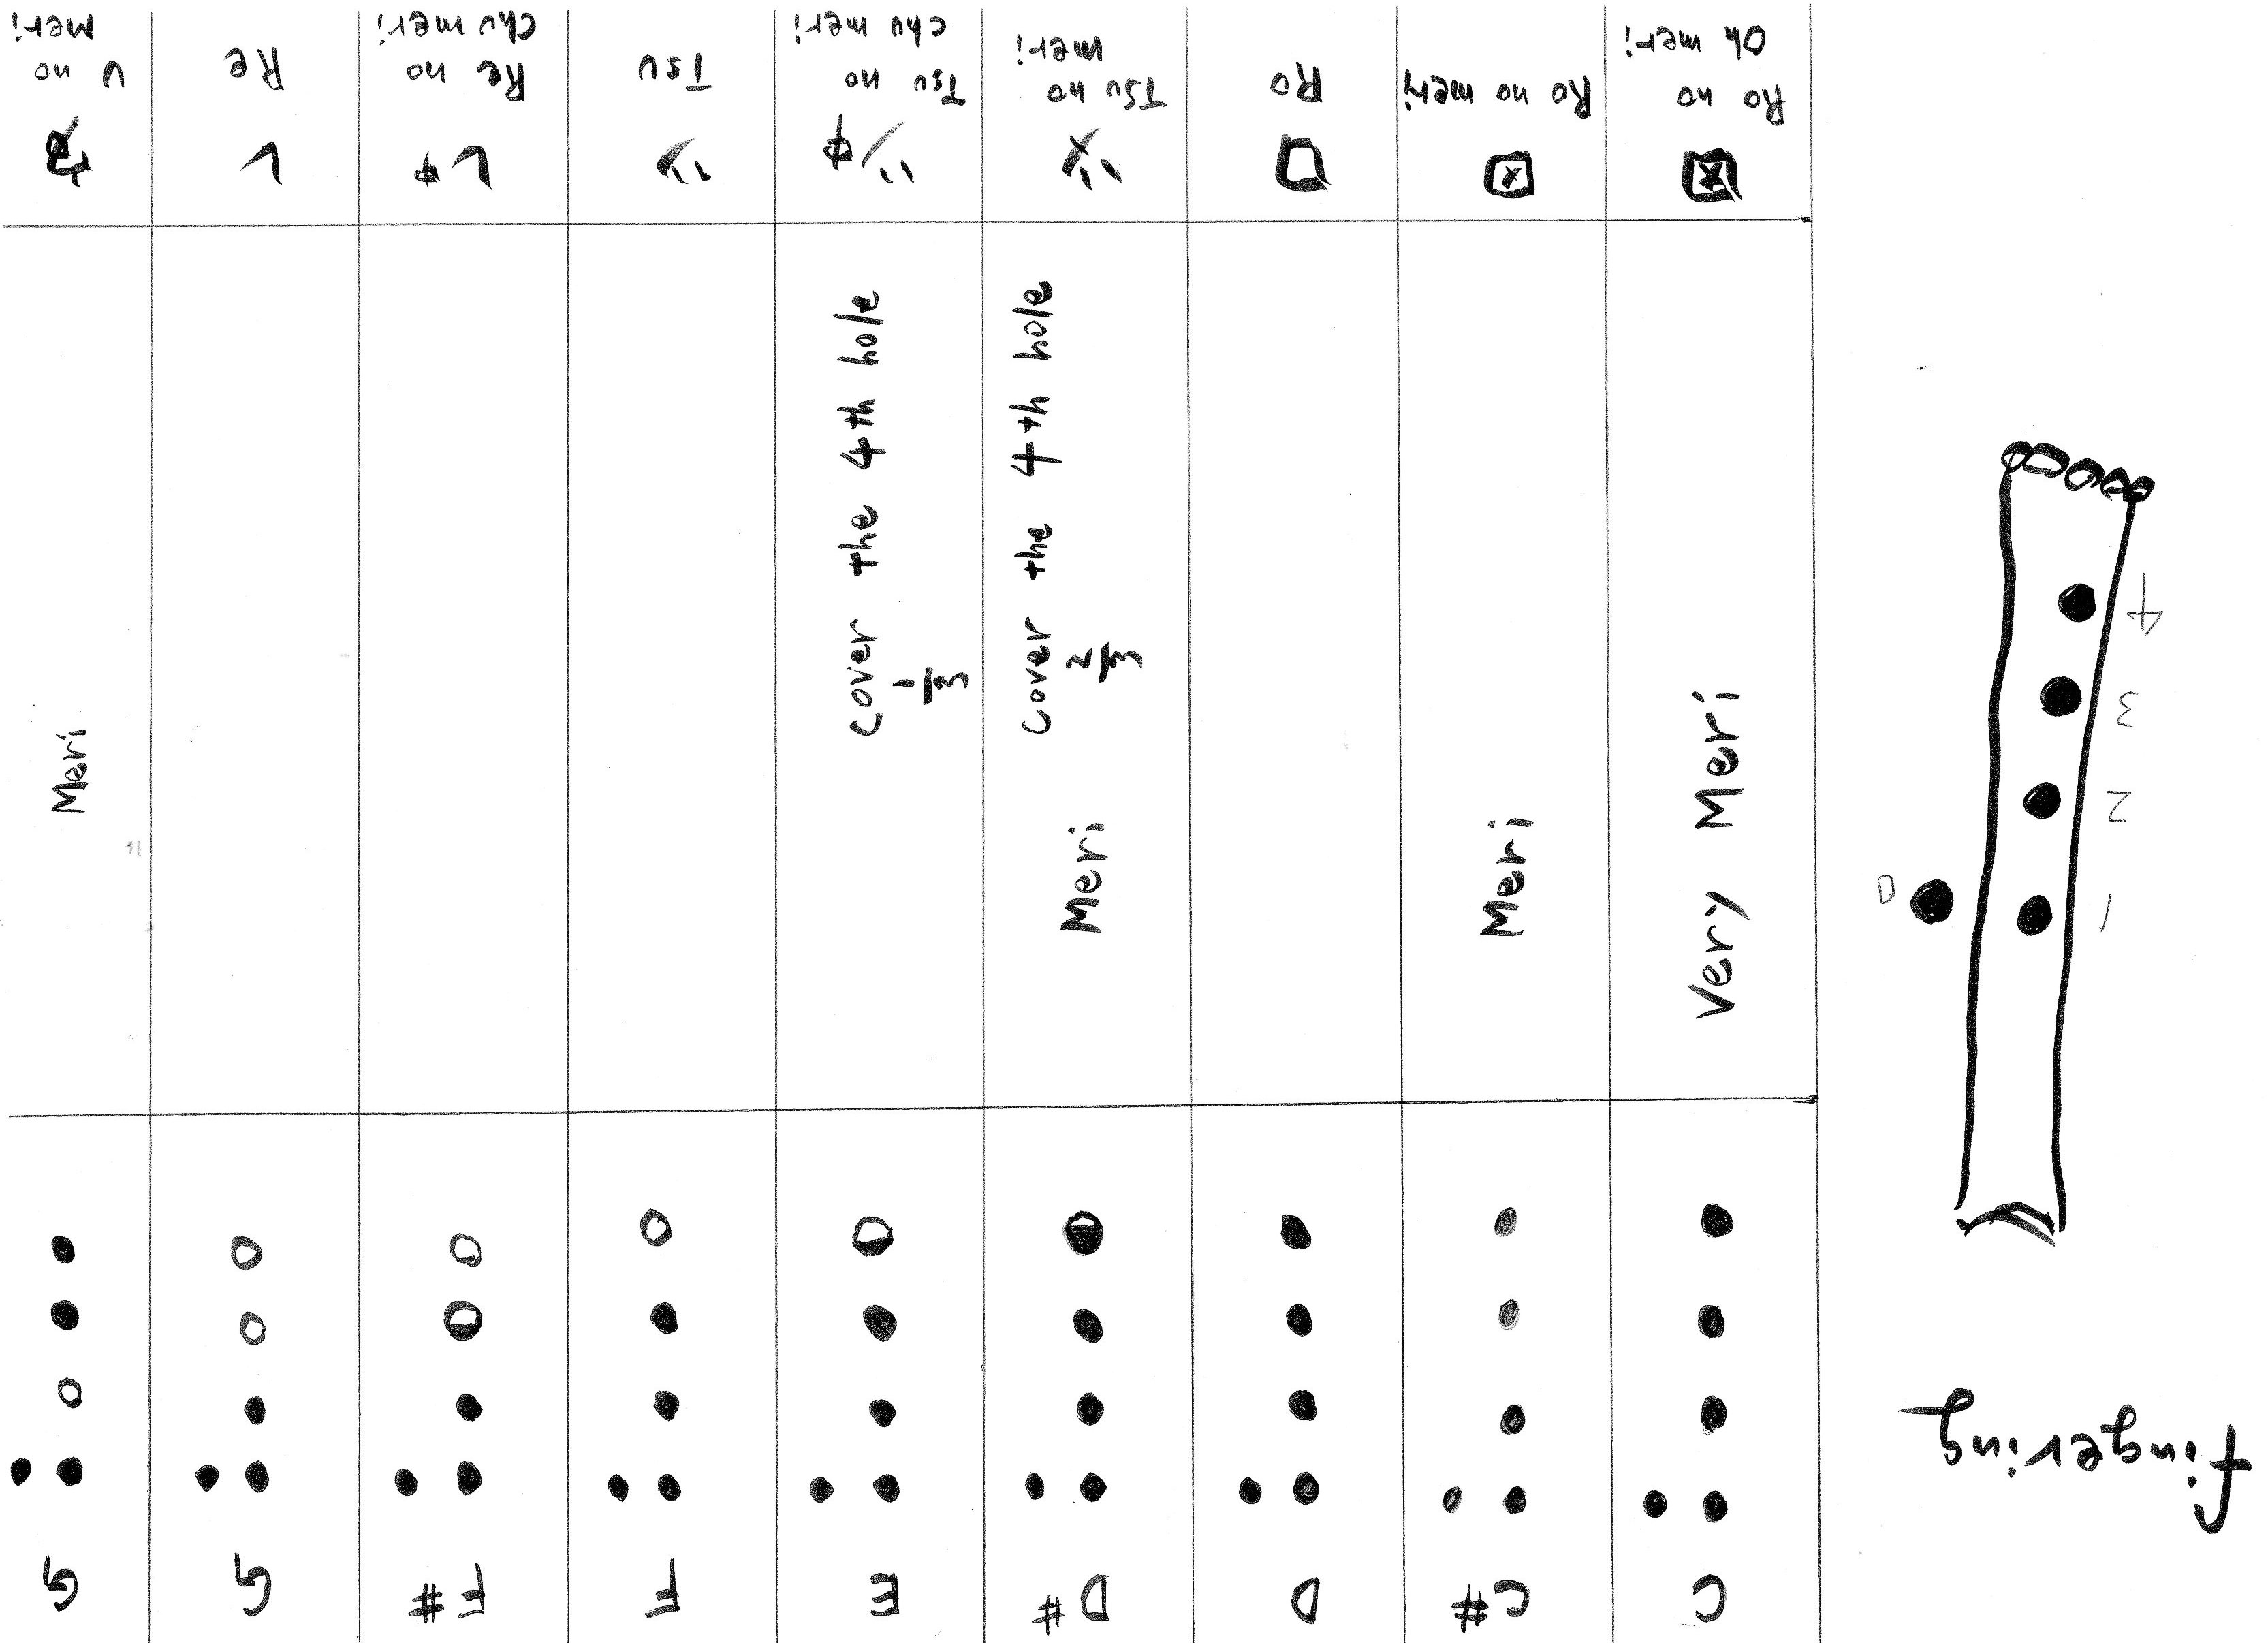
\includegraphics[angle=270,width=0.8\textwidth]{尺八の運指表1}
	% 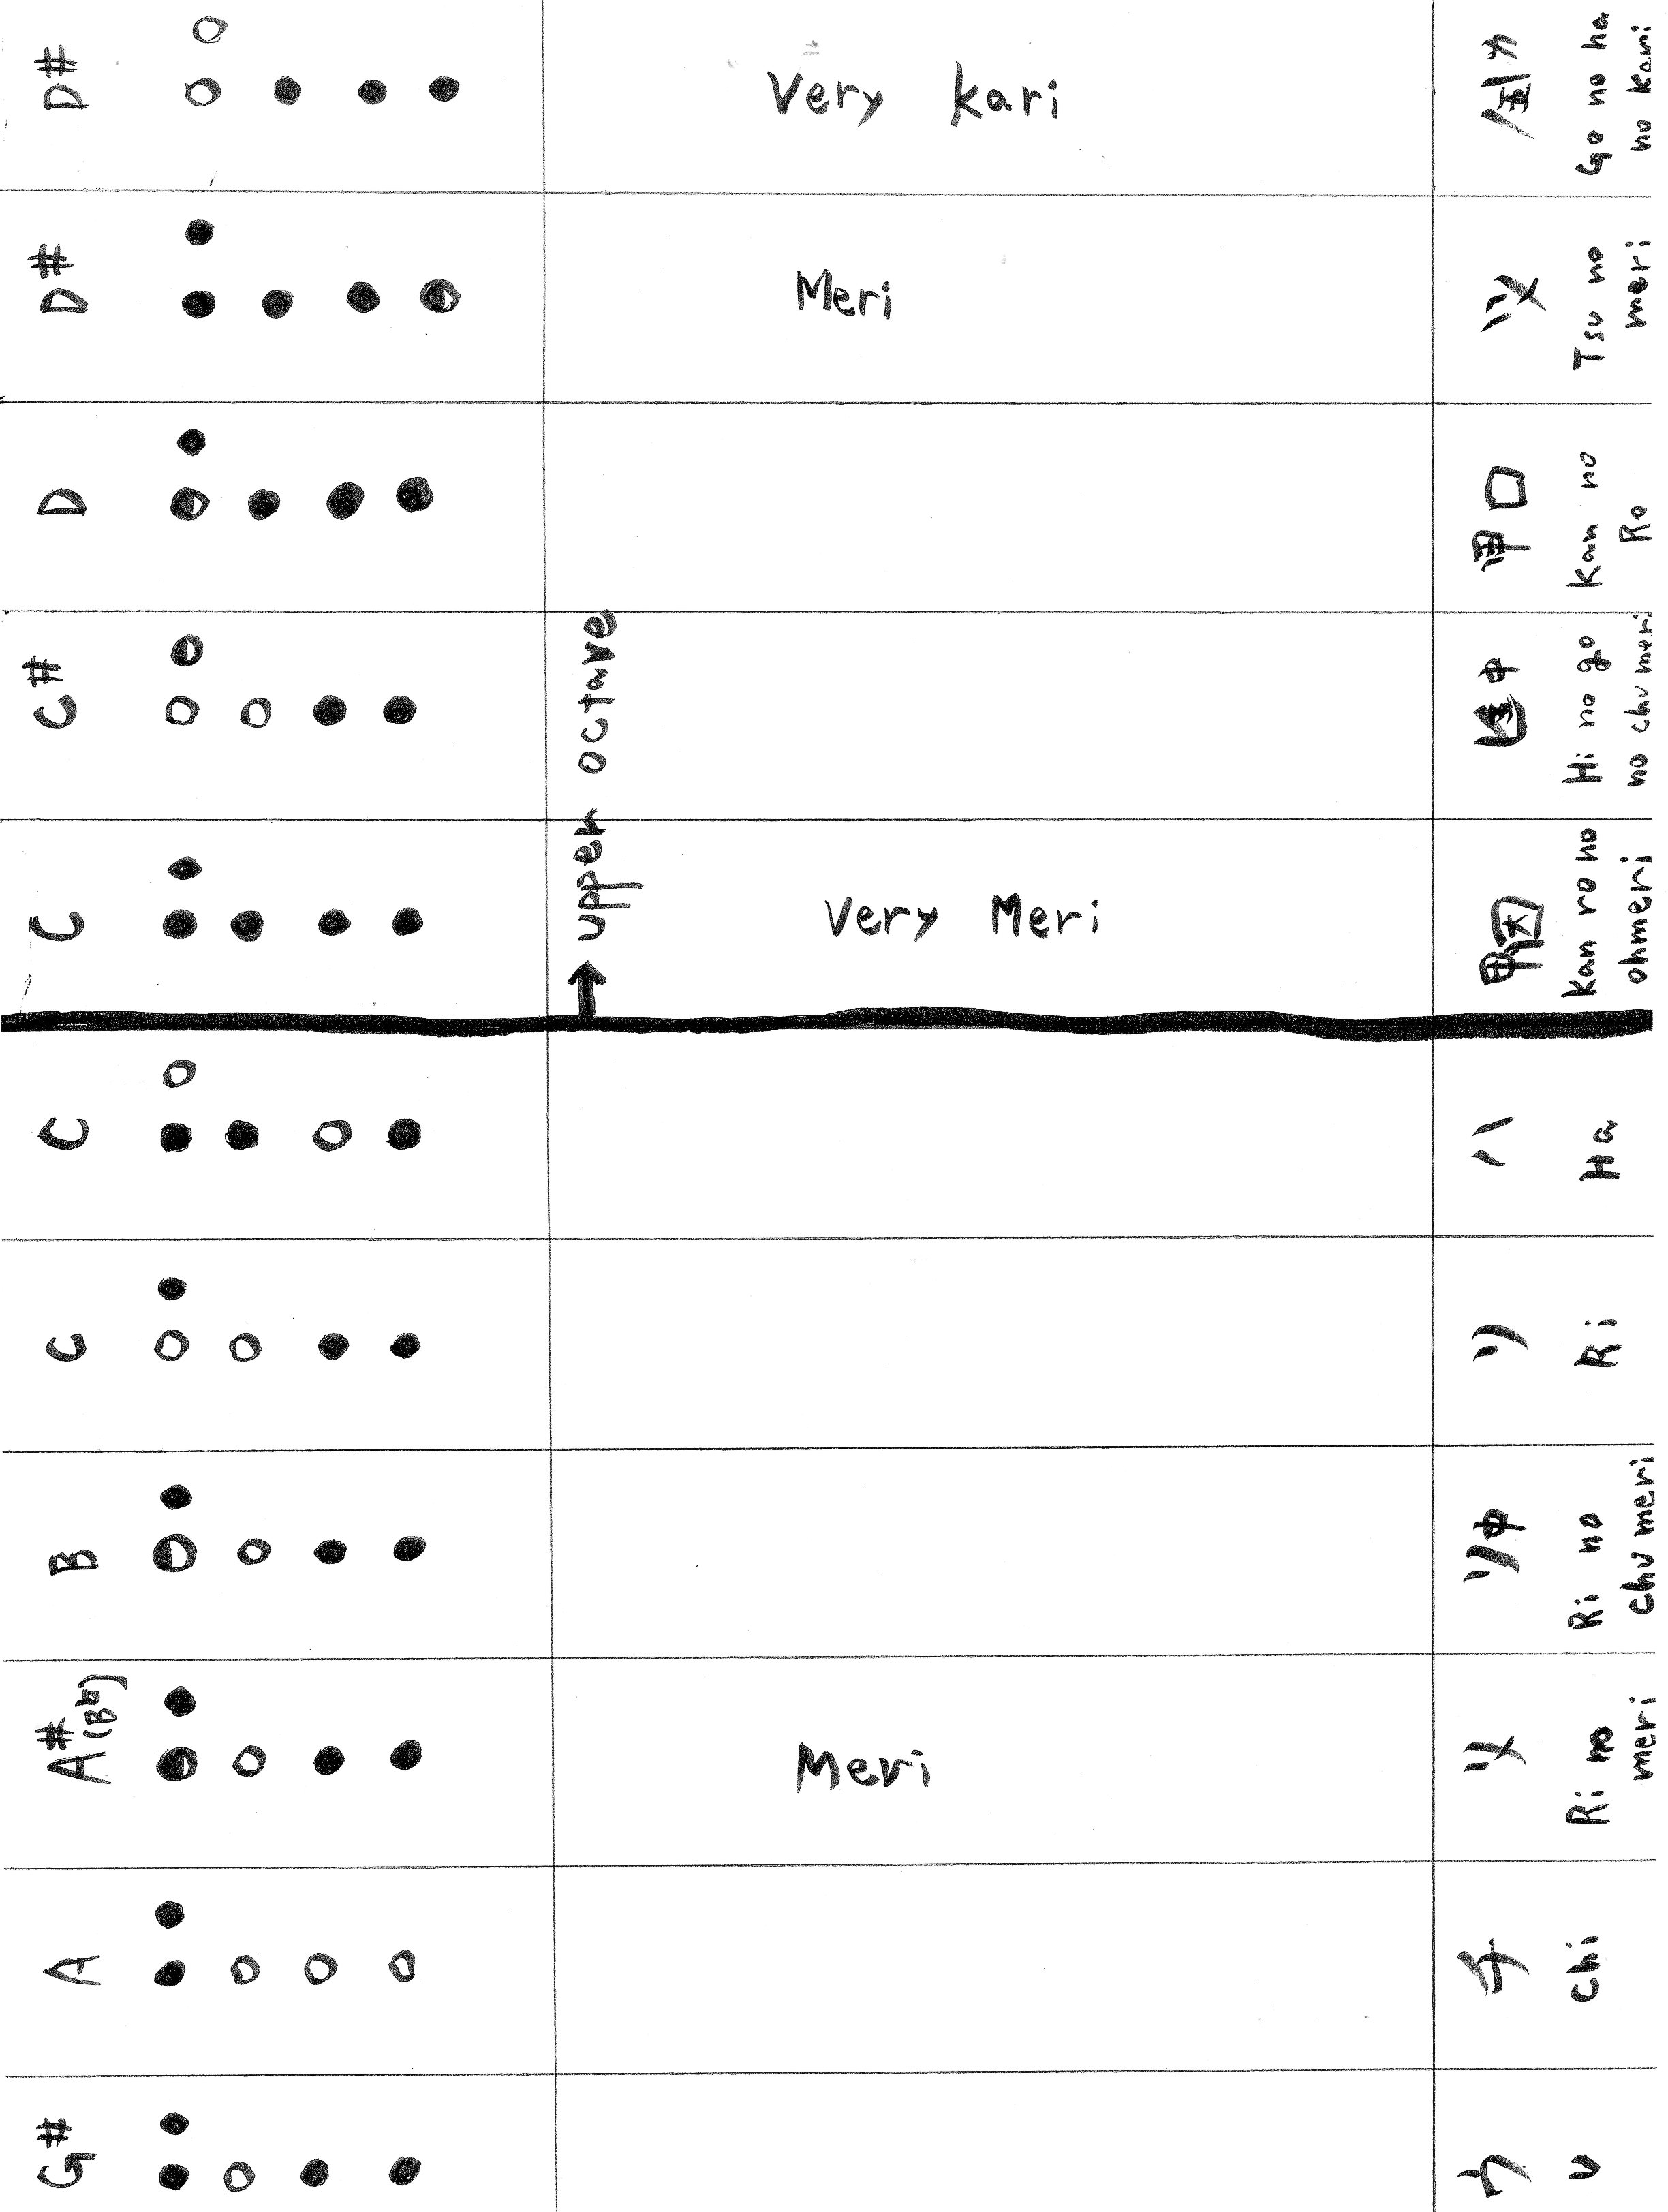
\includegraphics[width=0.8\textwidth,angle=270]{尺八の運指表2.jpg}
	% 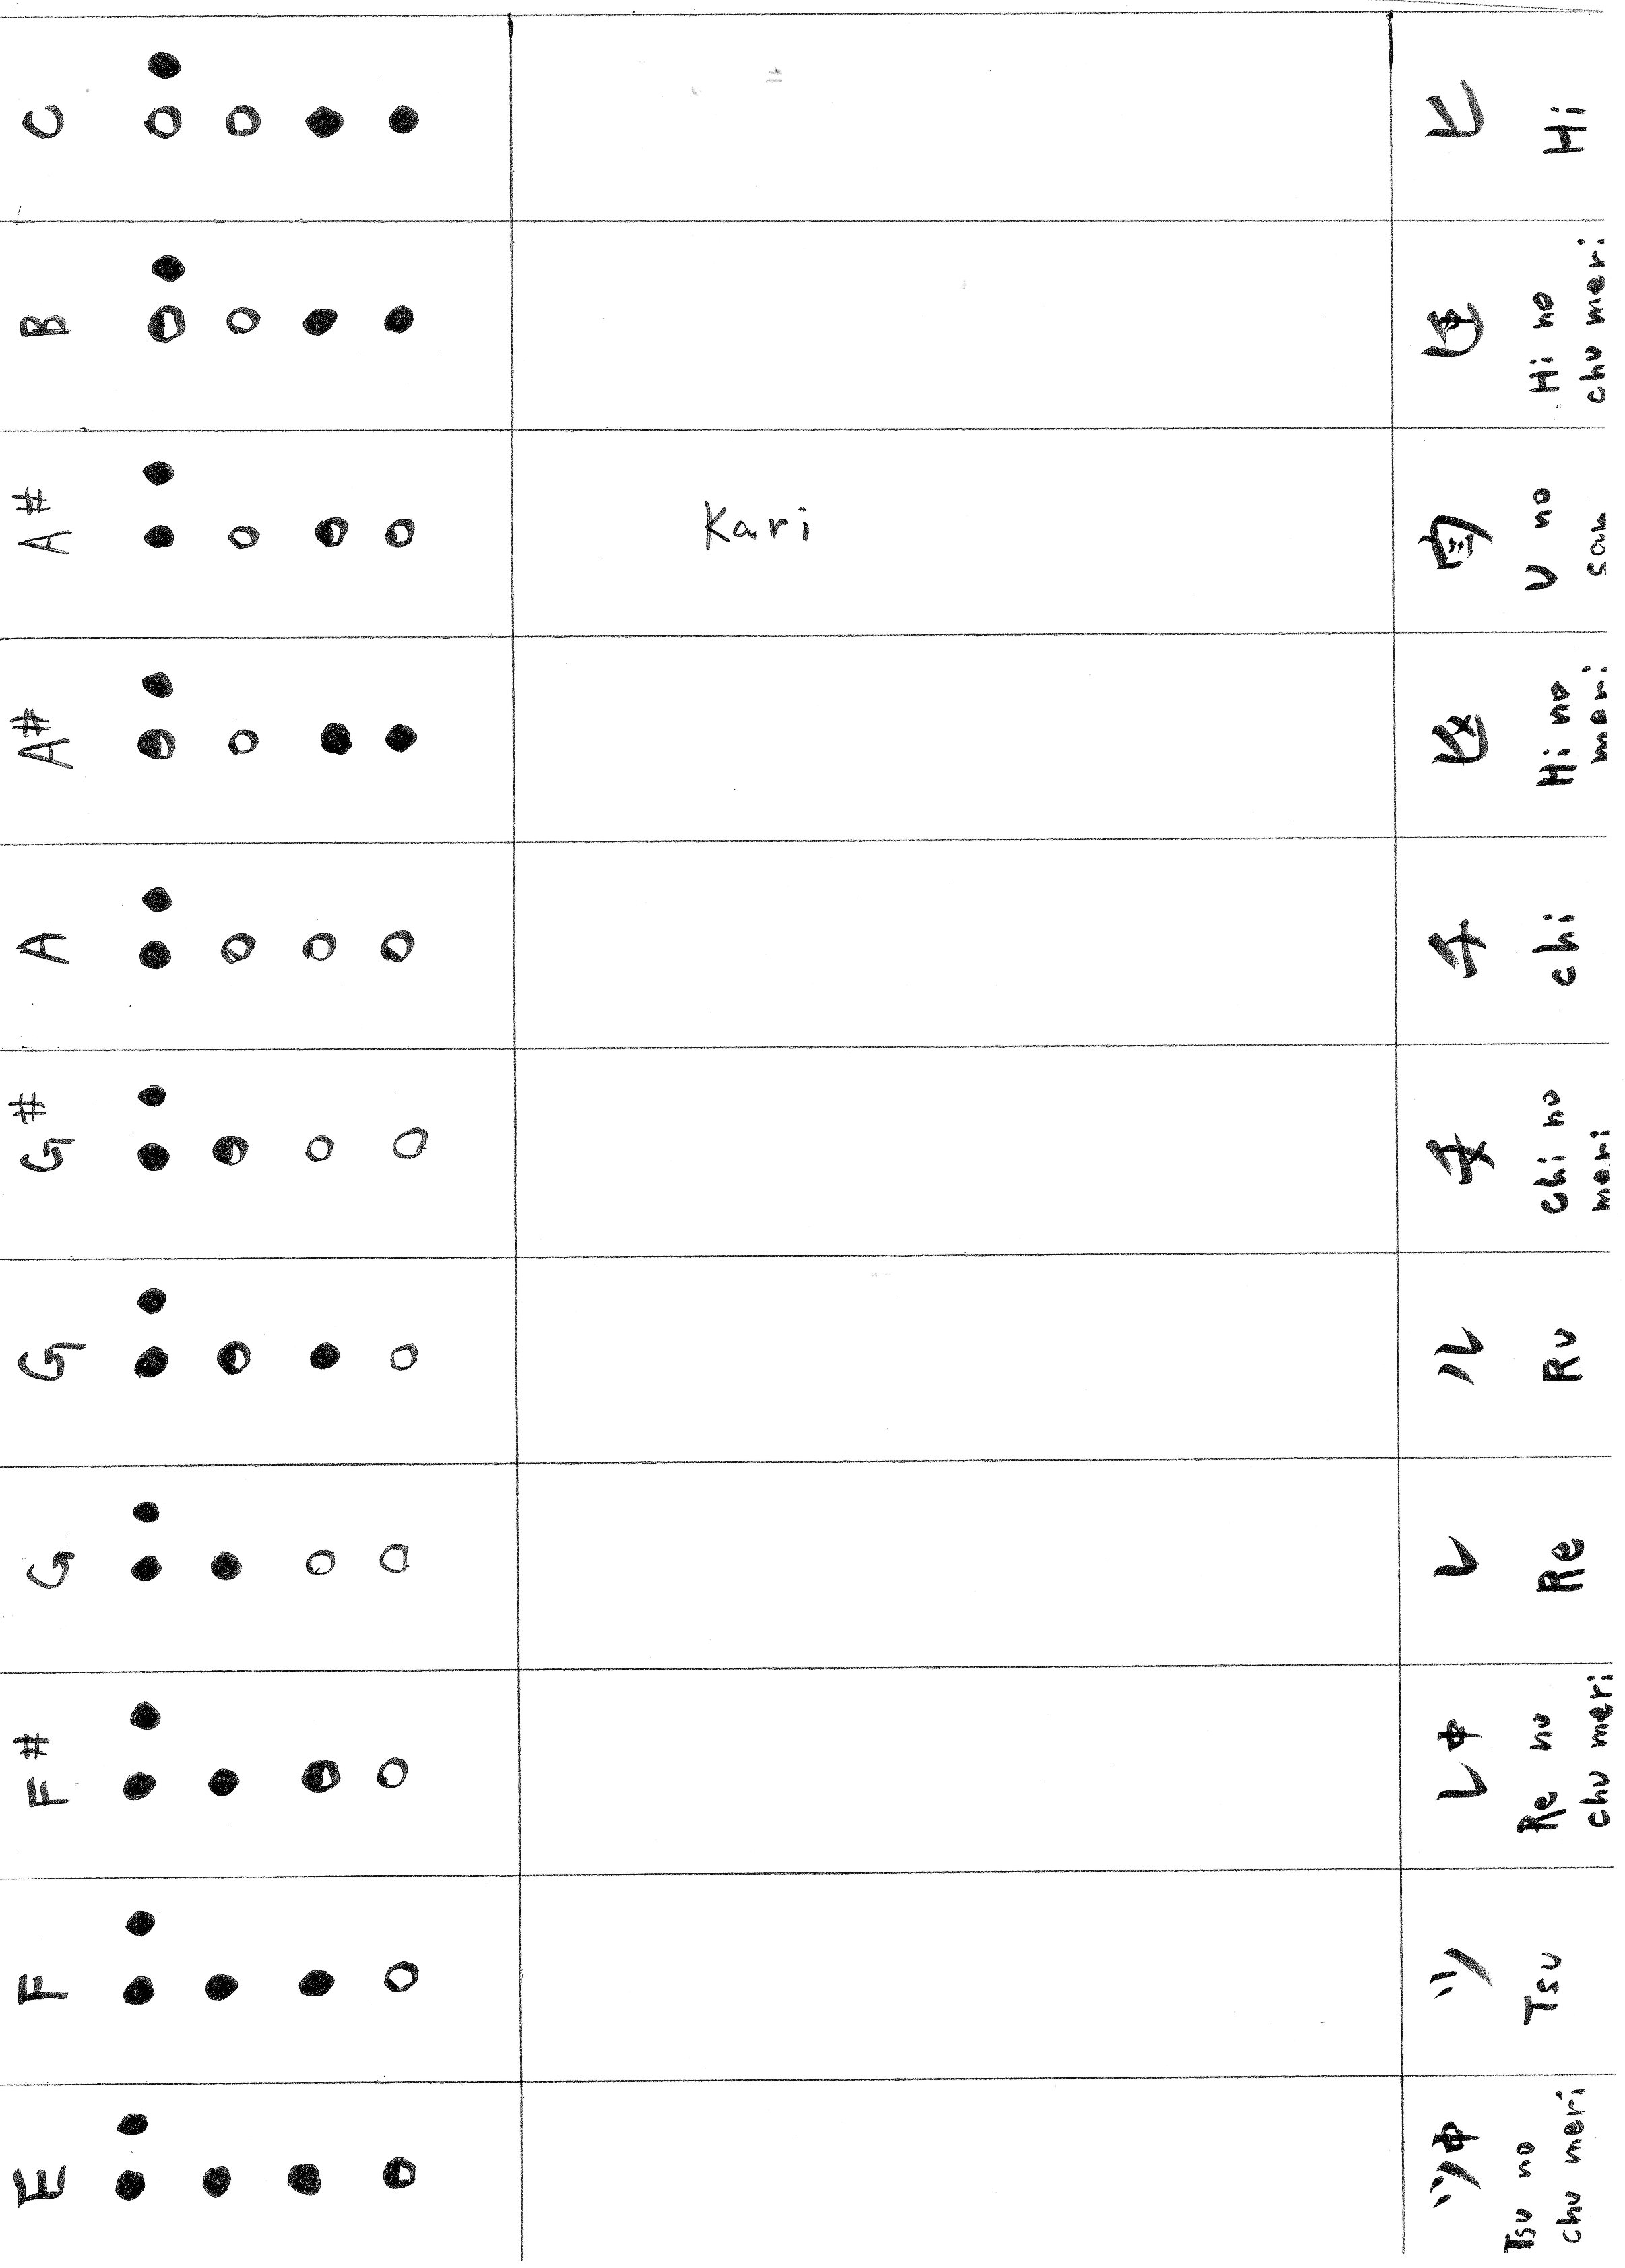
\includegraphics[width=0.8\textwidth,angle=270]{尺八の運指表3.jpg}
	% 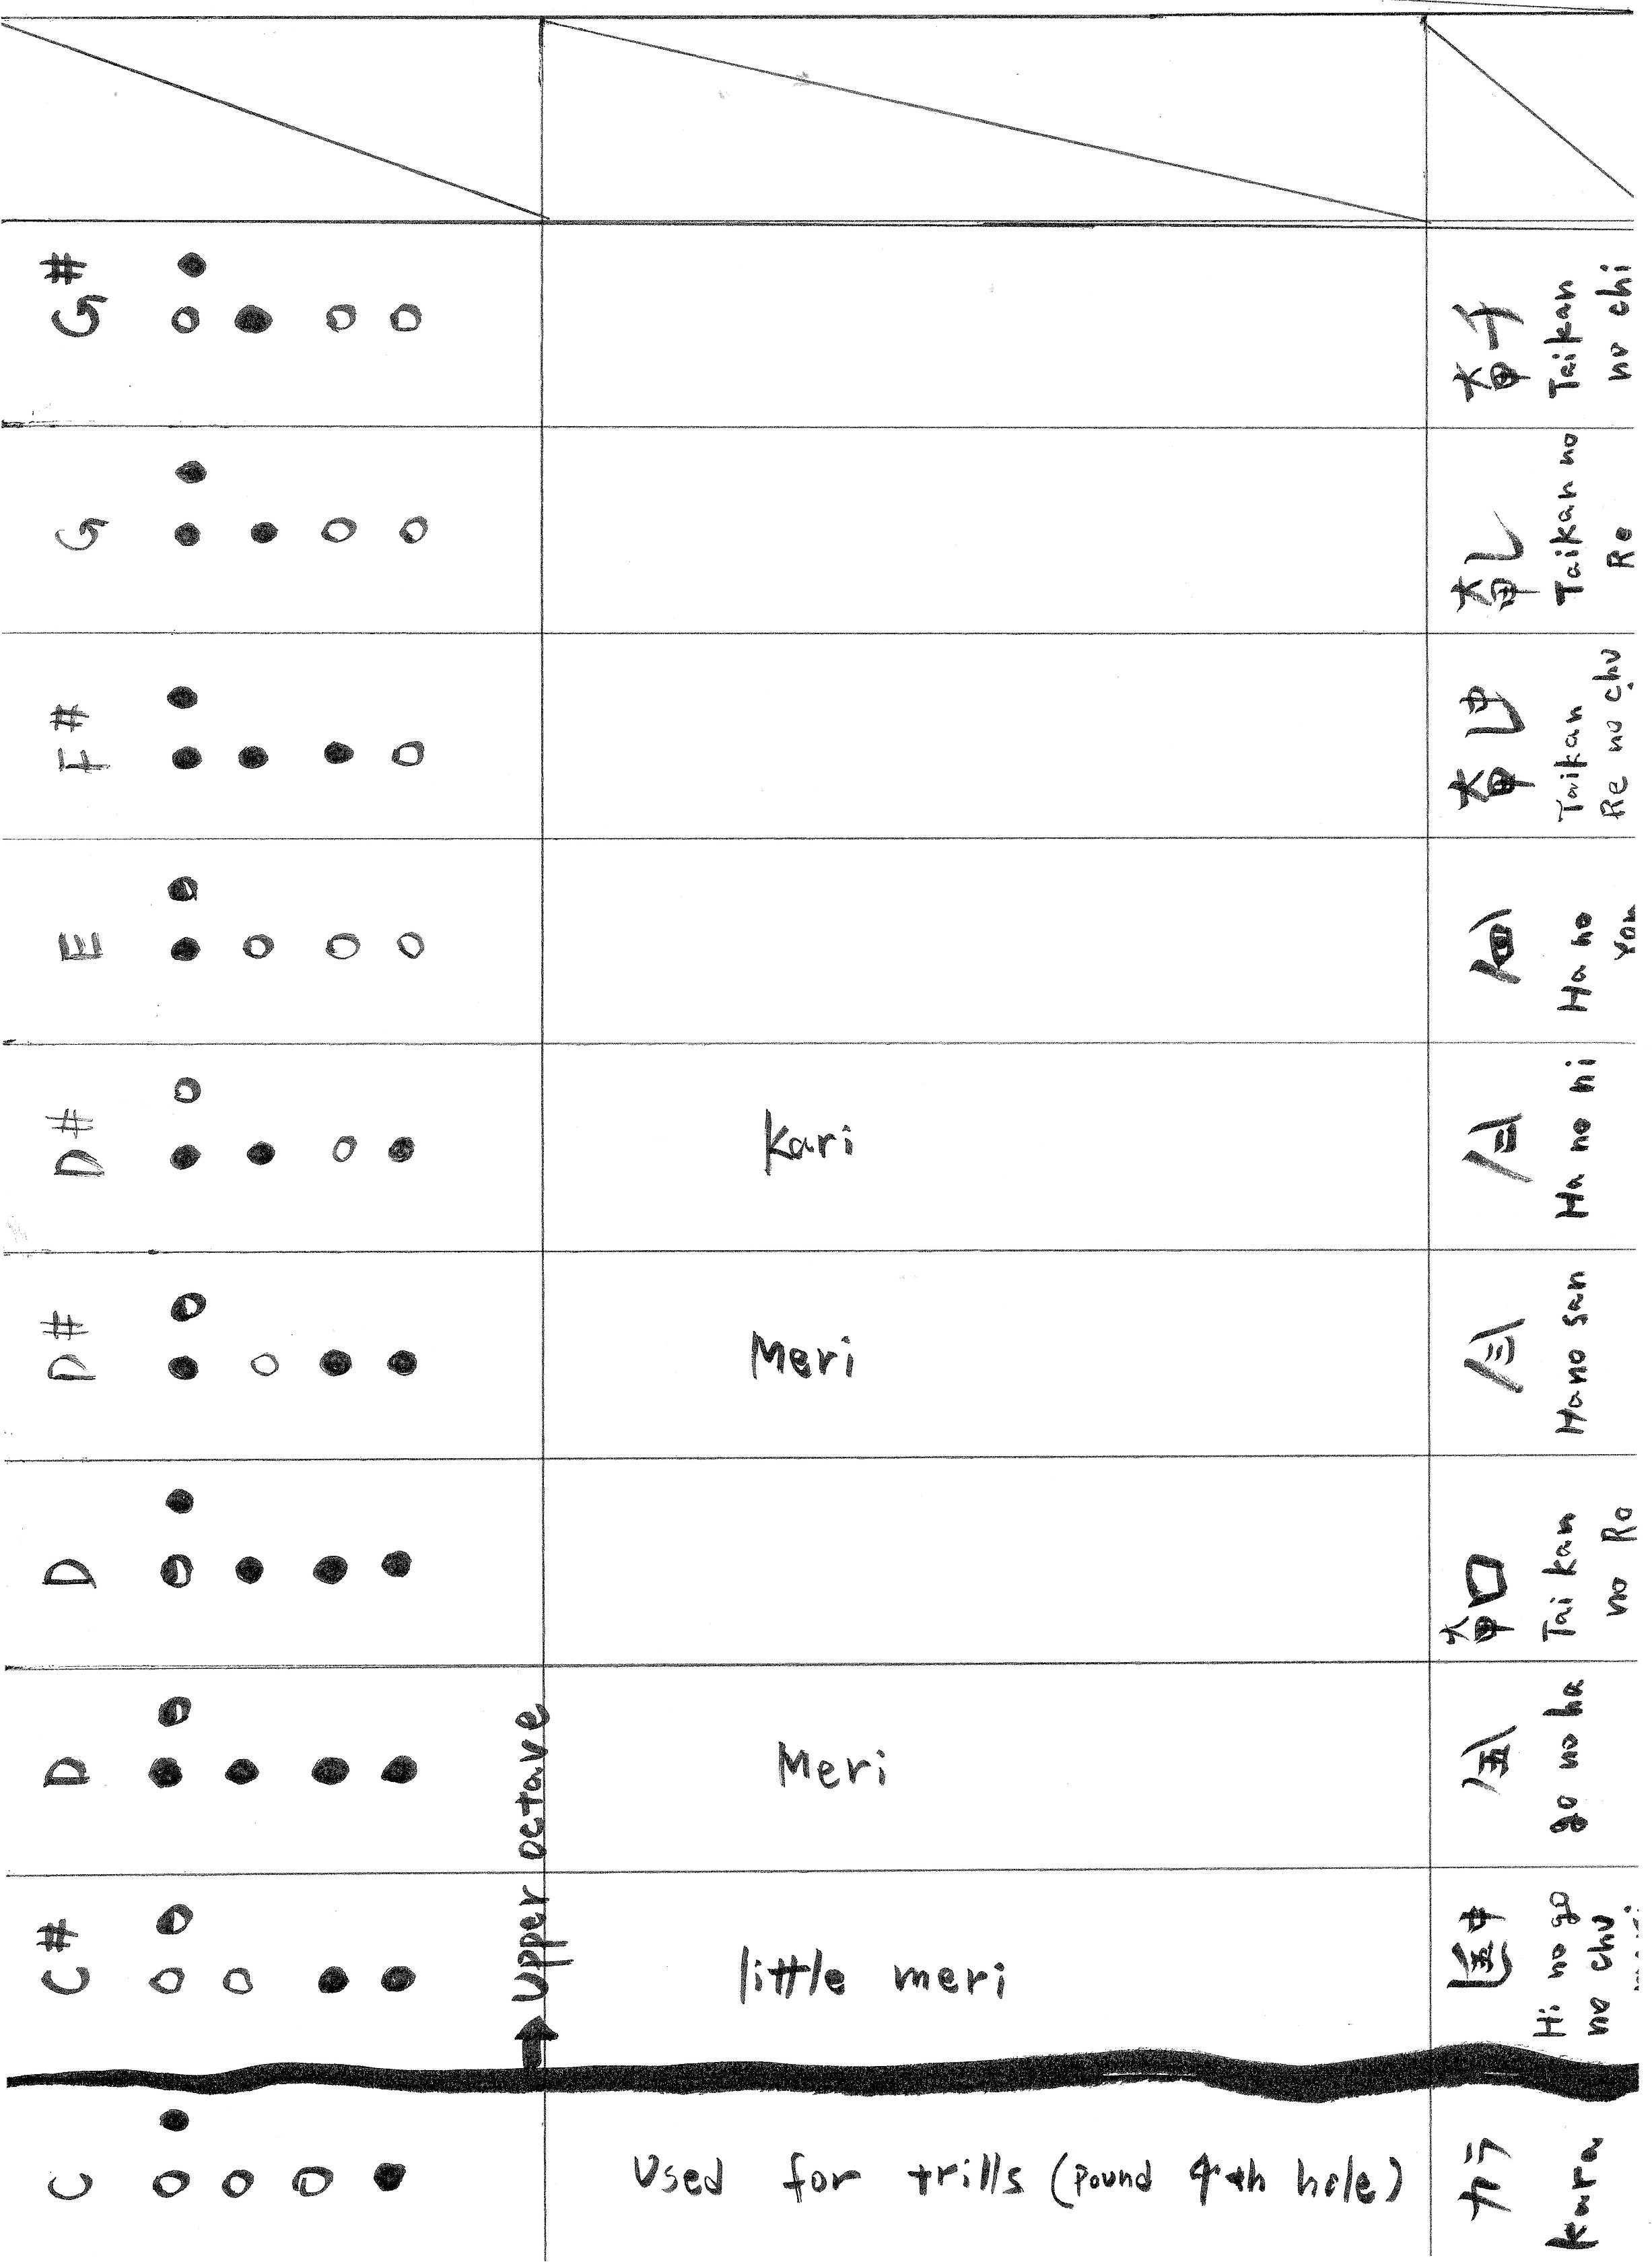
\includegraphics[width=0.8\textwidth,angle=270]{尺八の運指表4.jpg}
	\caption{Shakuhachi fingerings Part 0}
	\label{fig:shakuhachi_fingerings_0}
\end{figure}

\begin{figure}[p]
	\centering
	% 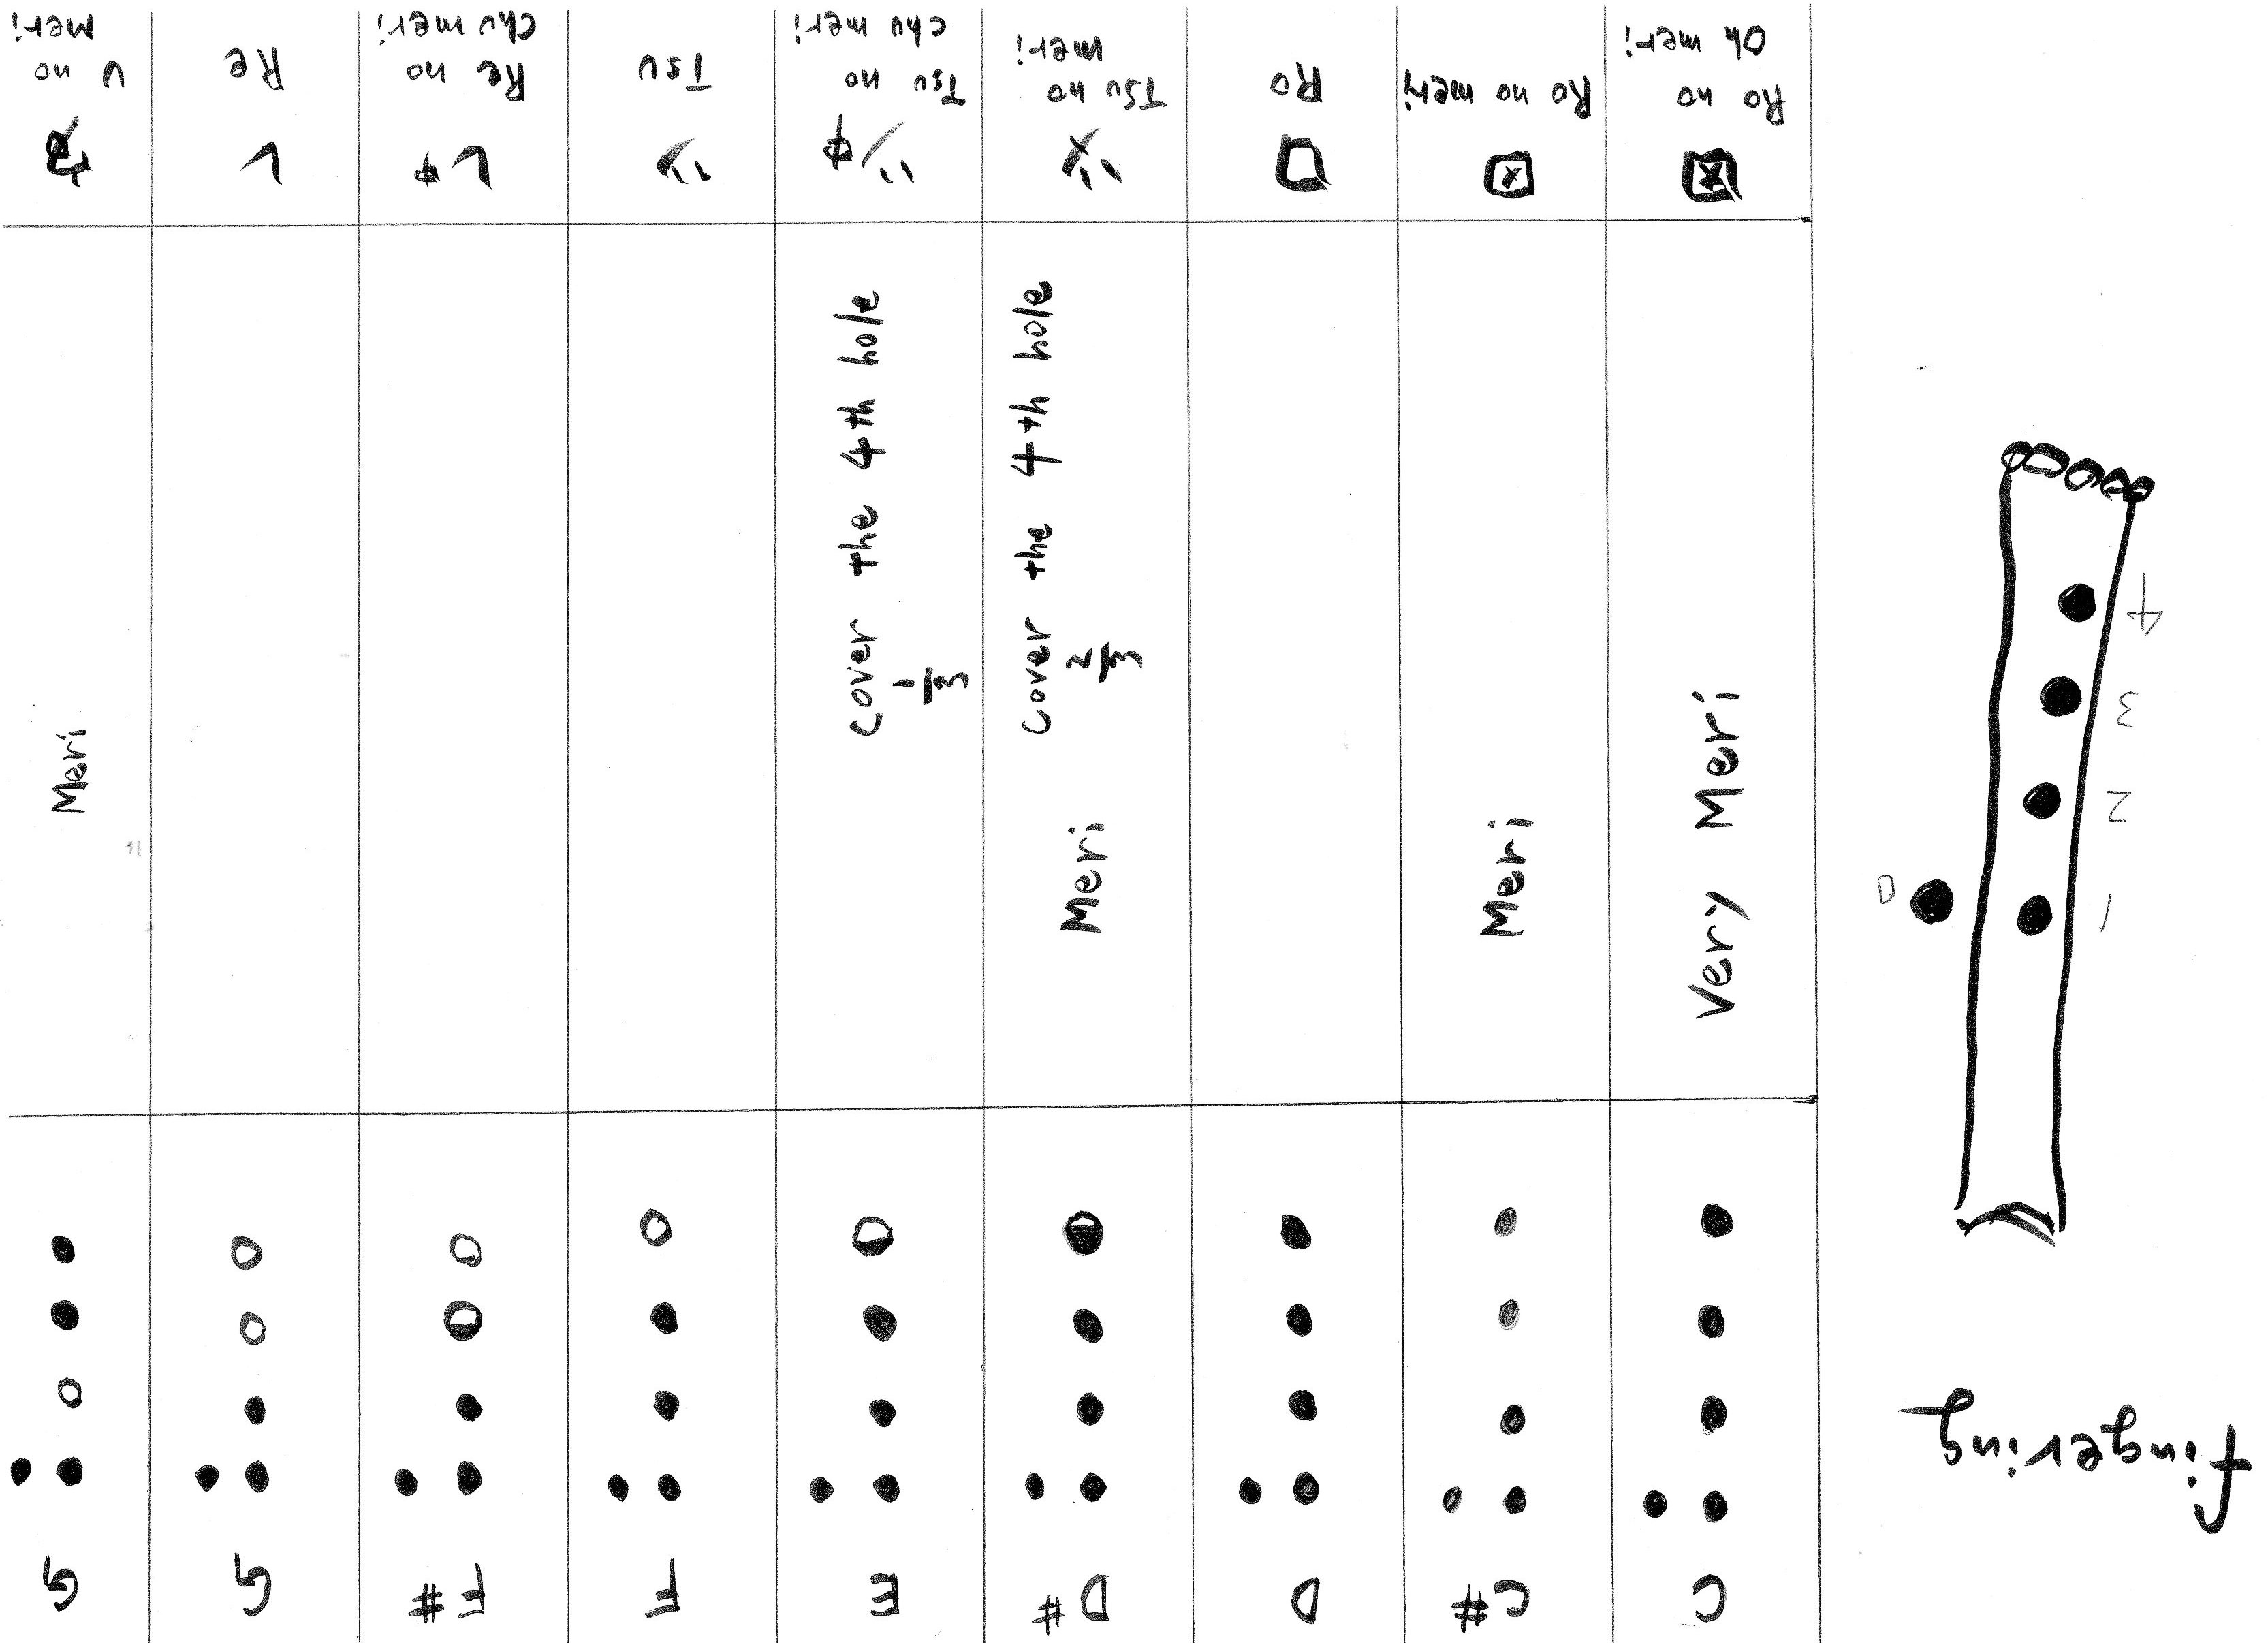
\includegraphics[width=0.8\textwidth,angle=270]{尺八の運指表1.jpg}
	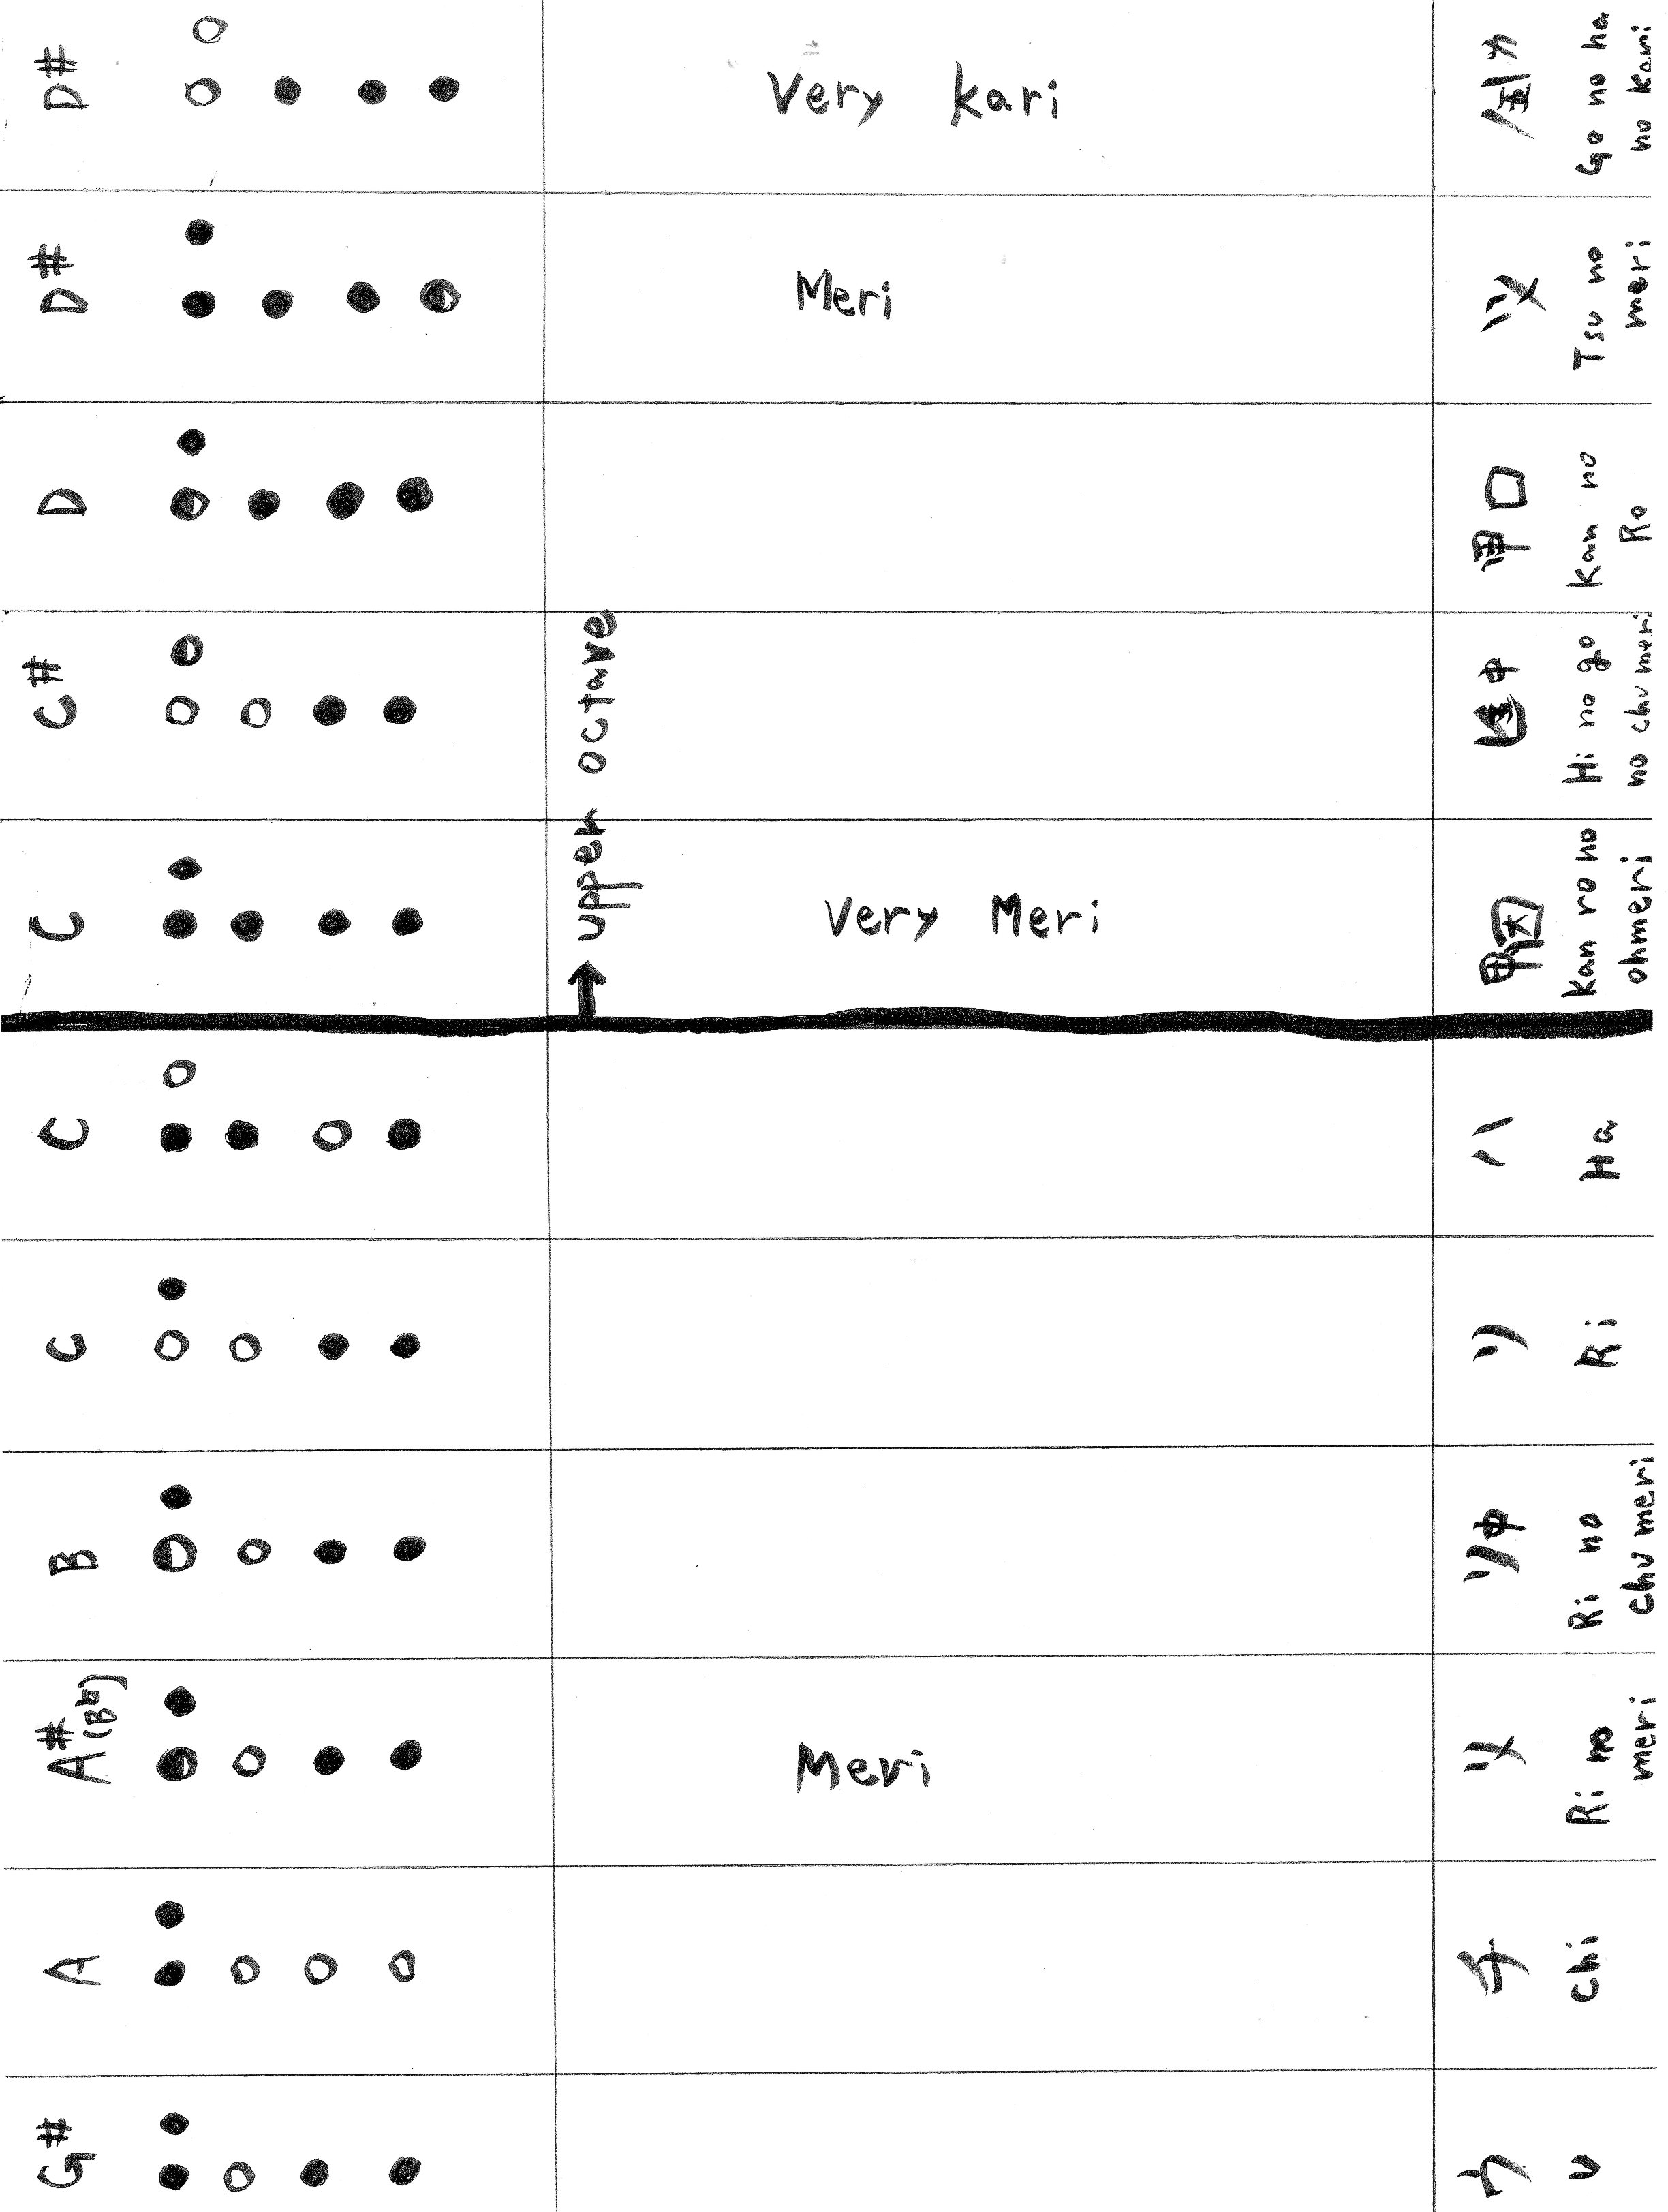
\includegraphics[width=0.8\textwidth,angle=270]{尺八の運指表2.jpg}
	% 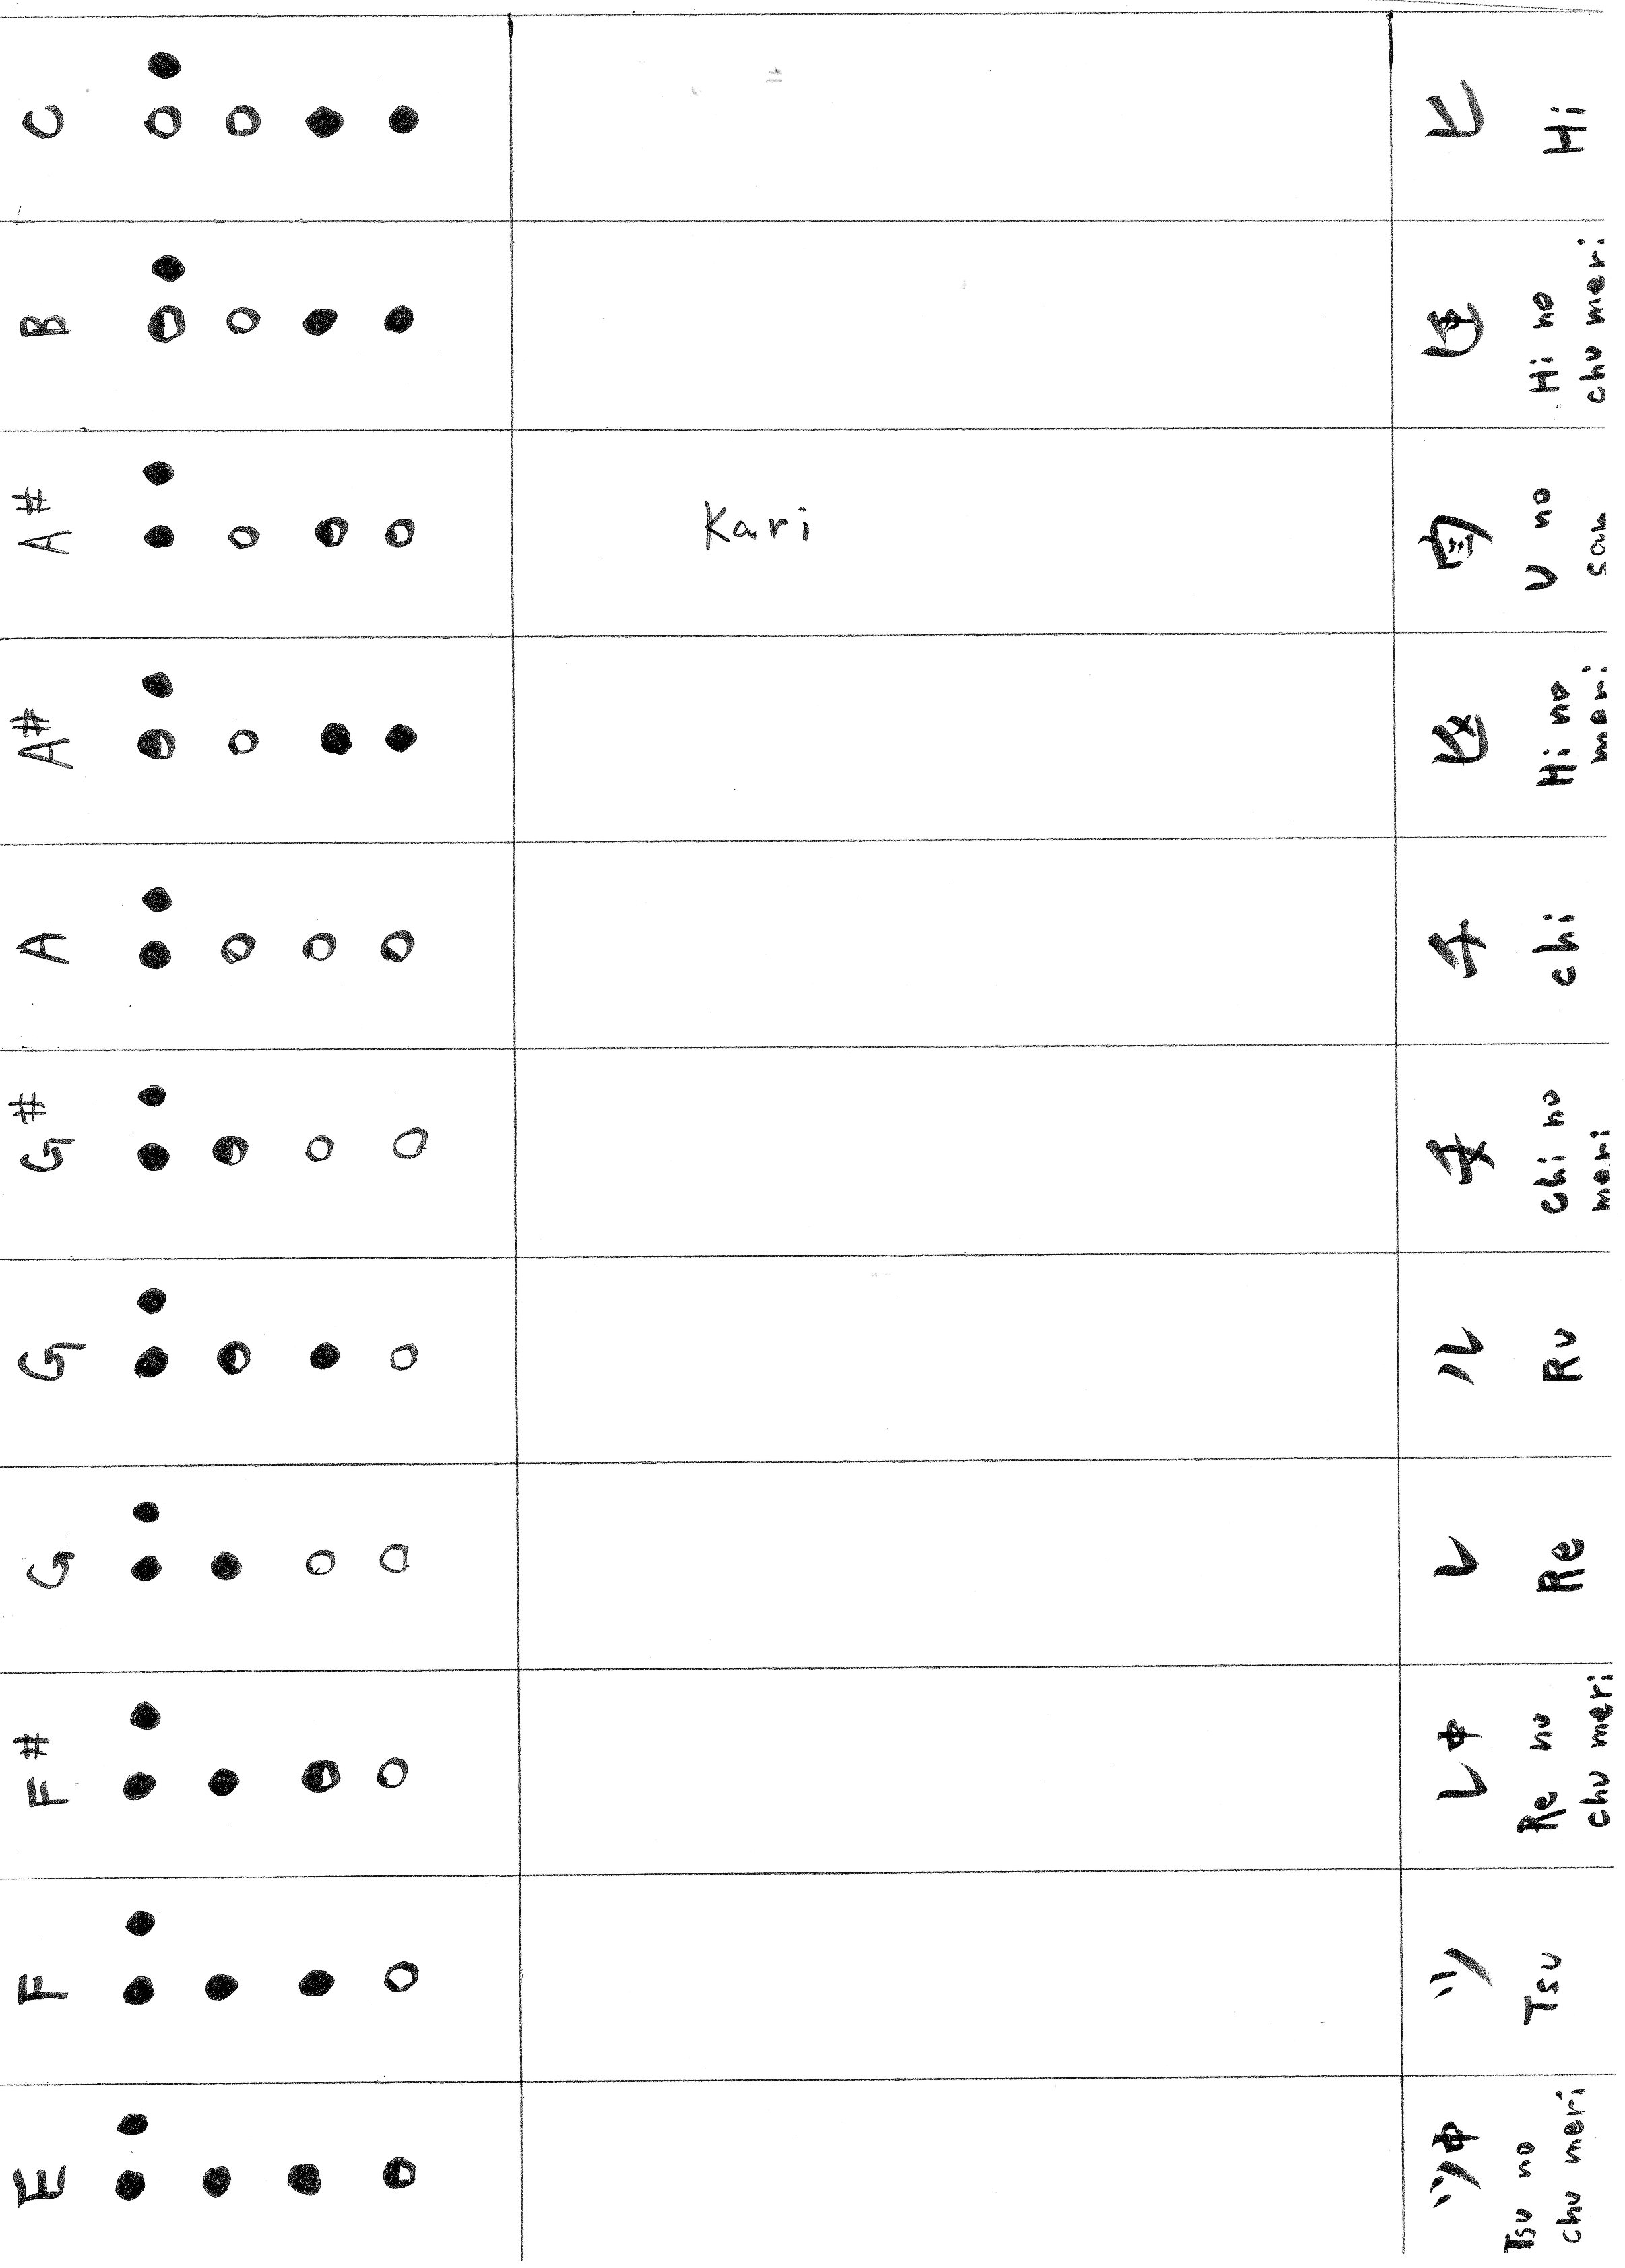
\includegraphics[width=0.8\textwidth,angle=270]{尺八の運指表3.jpg}
	% 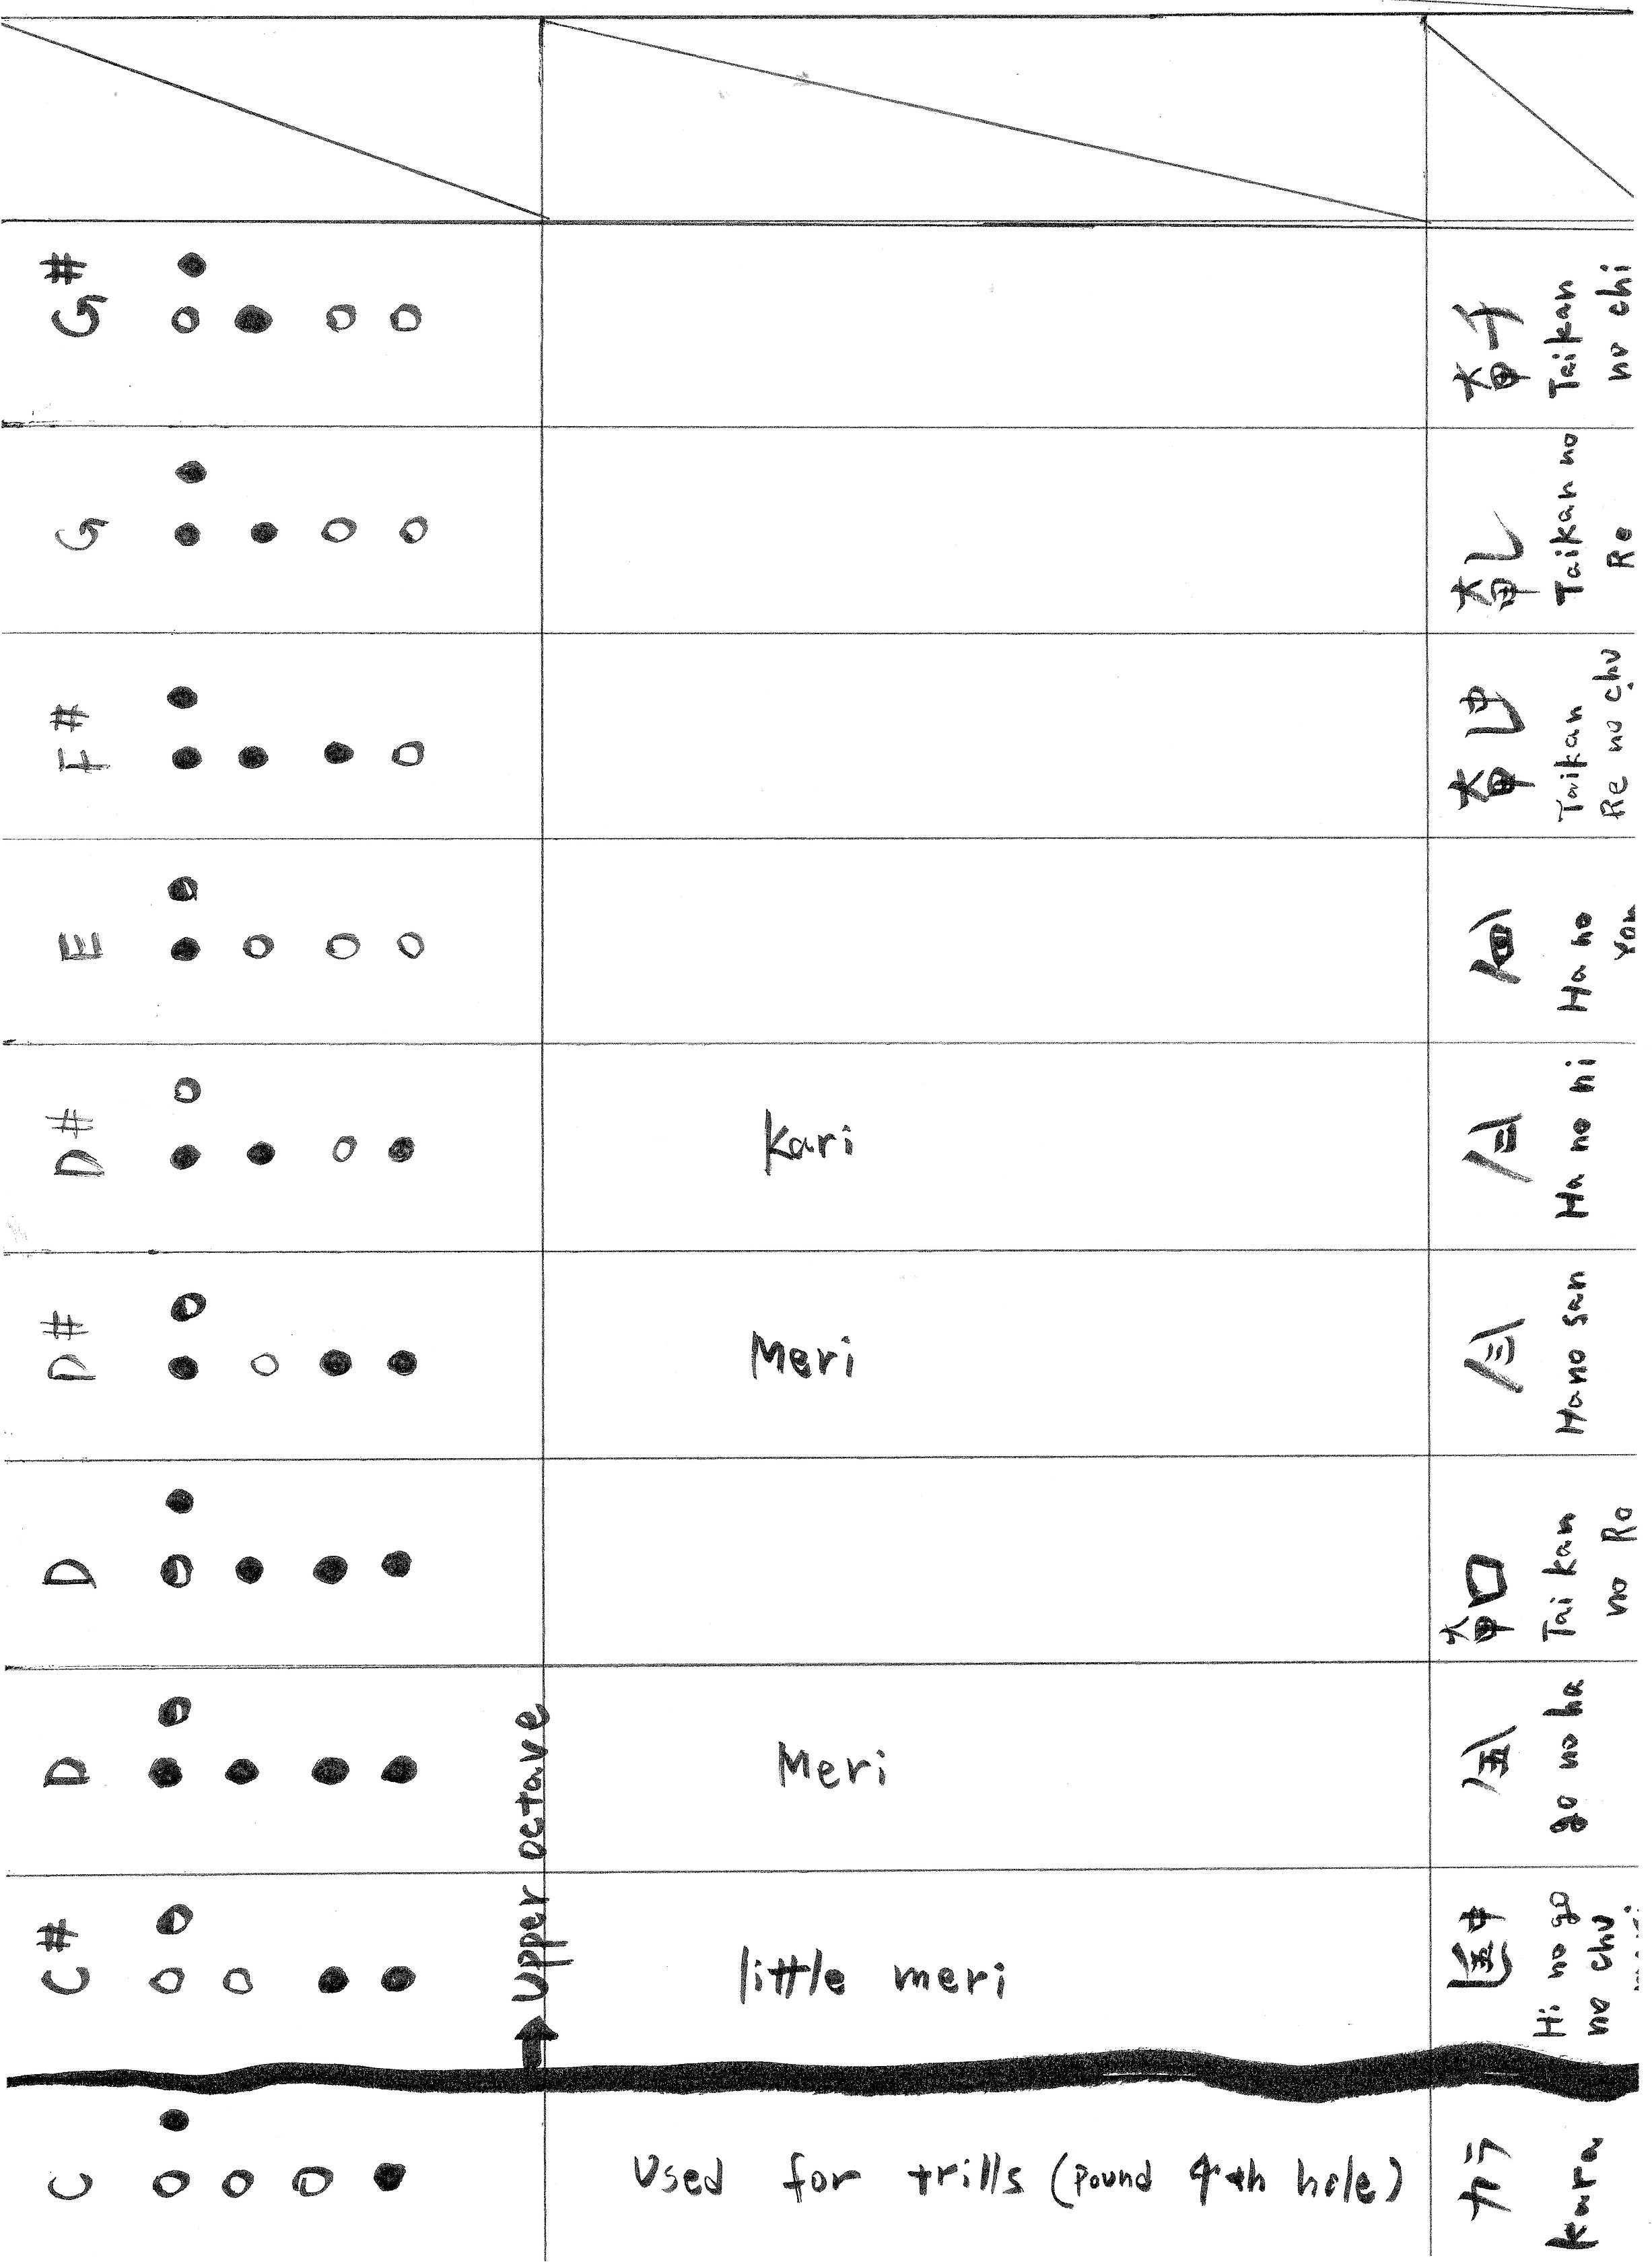
\includegraphics[width=0.8\textwidth,angle=270]{尺八の運指表4.jpg}
	\caption{Shakuhachi fingerings Part 1}
	\label{fig:shakuhachi_fingerings_1}
\end{figure}

\begin{figure}[p]
	\centering
	% 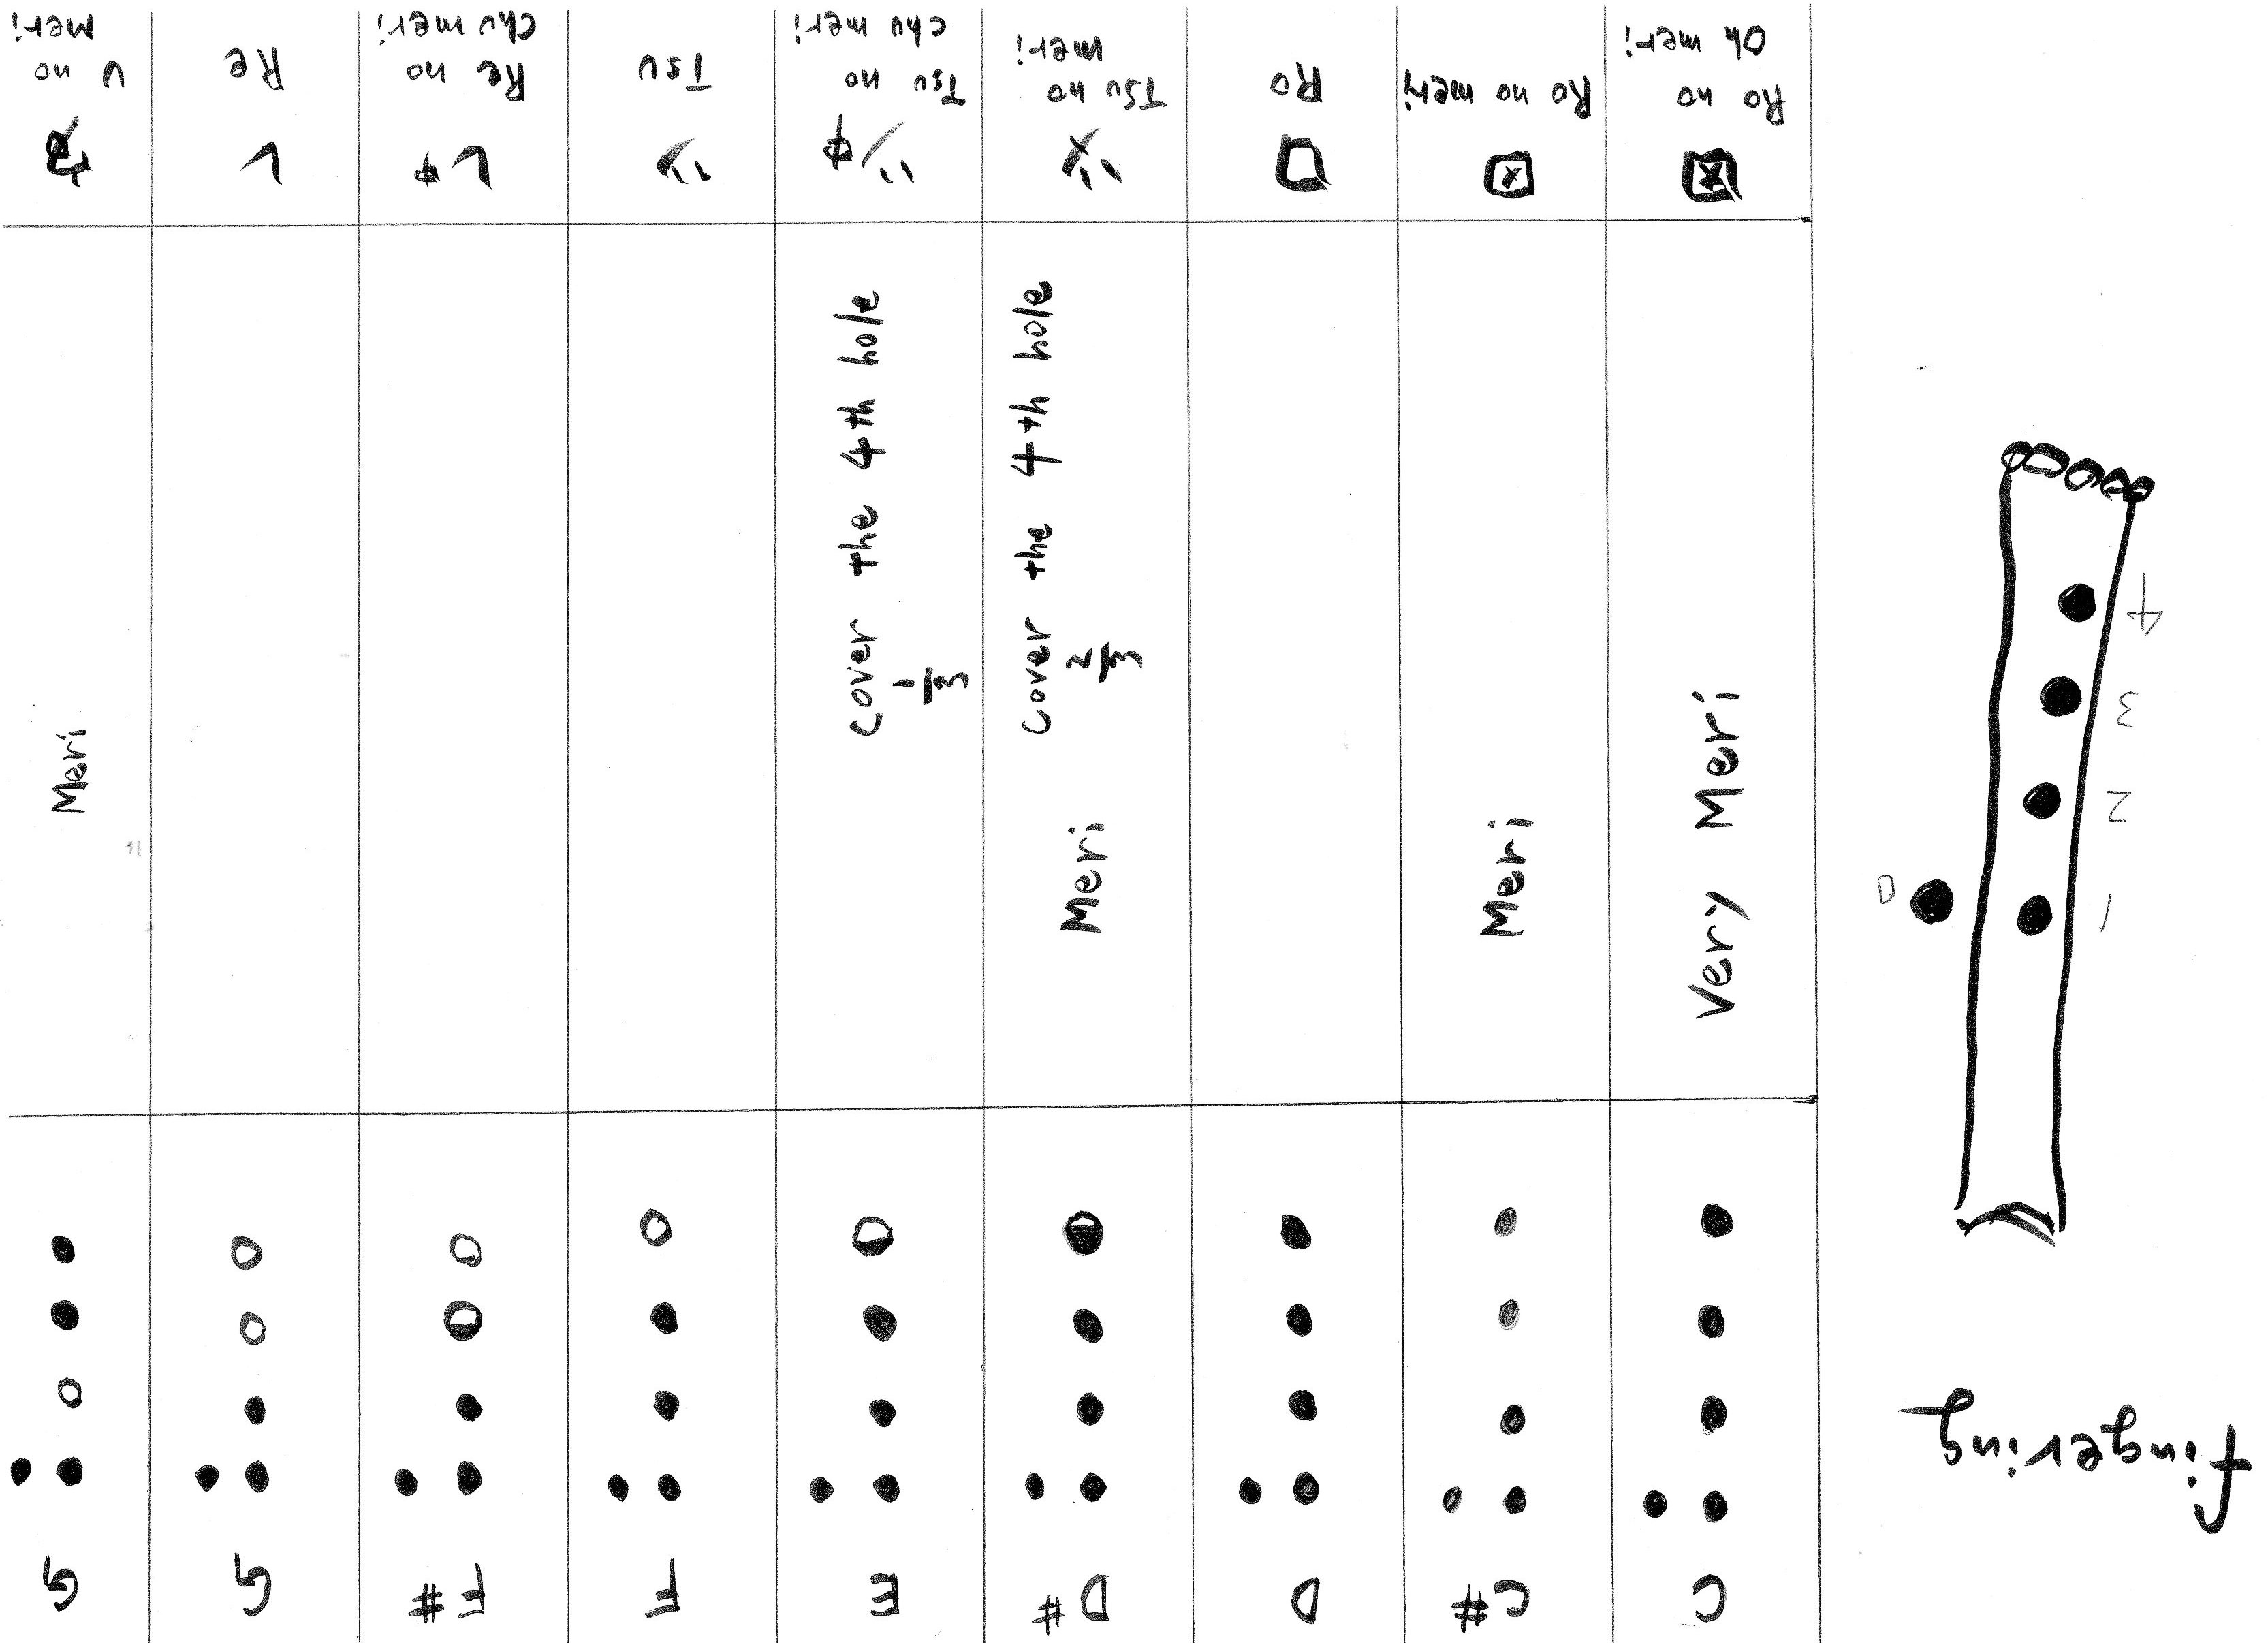
\includegraphics[width=0.8\textwidth,angle=270]{尺八の運指表1.jpg}
	% 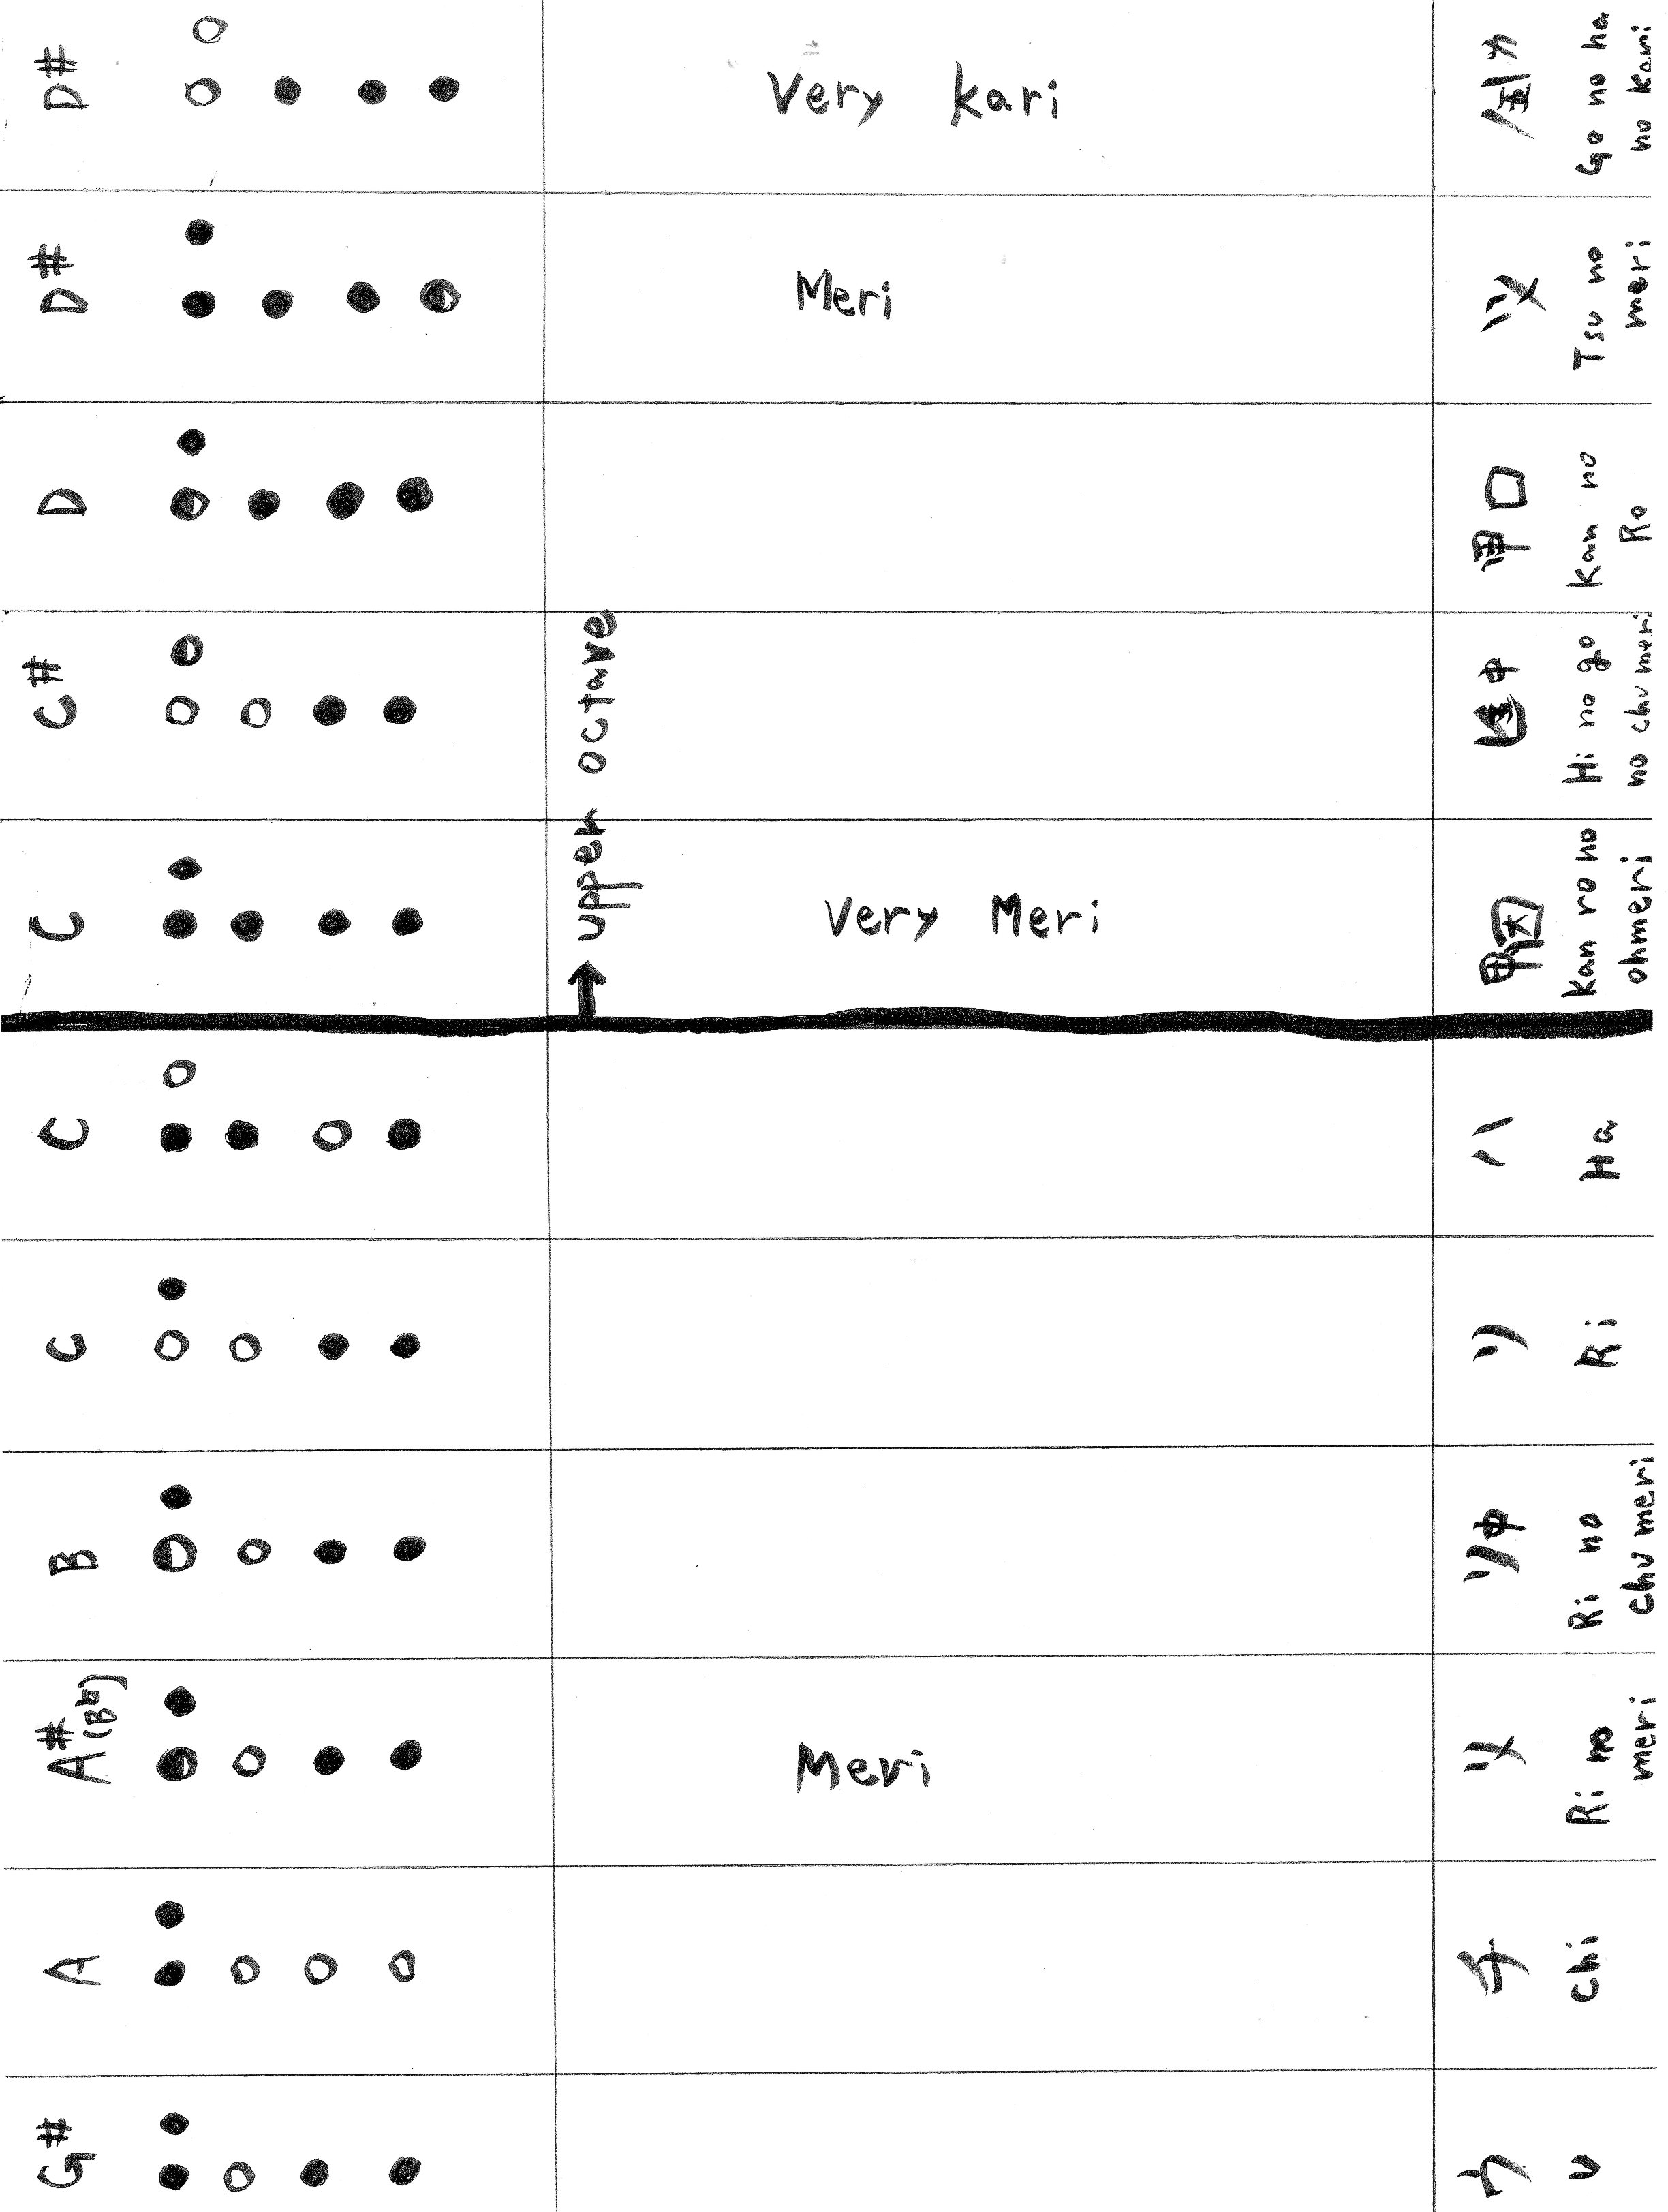
\includegraphics[width=0.8\textwidth,angle=270]{尺八の運指表2.jpg}
	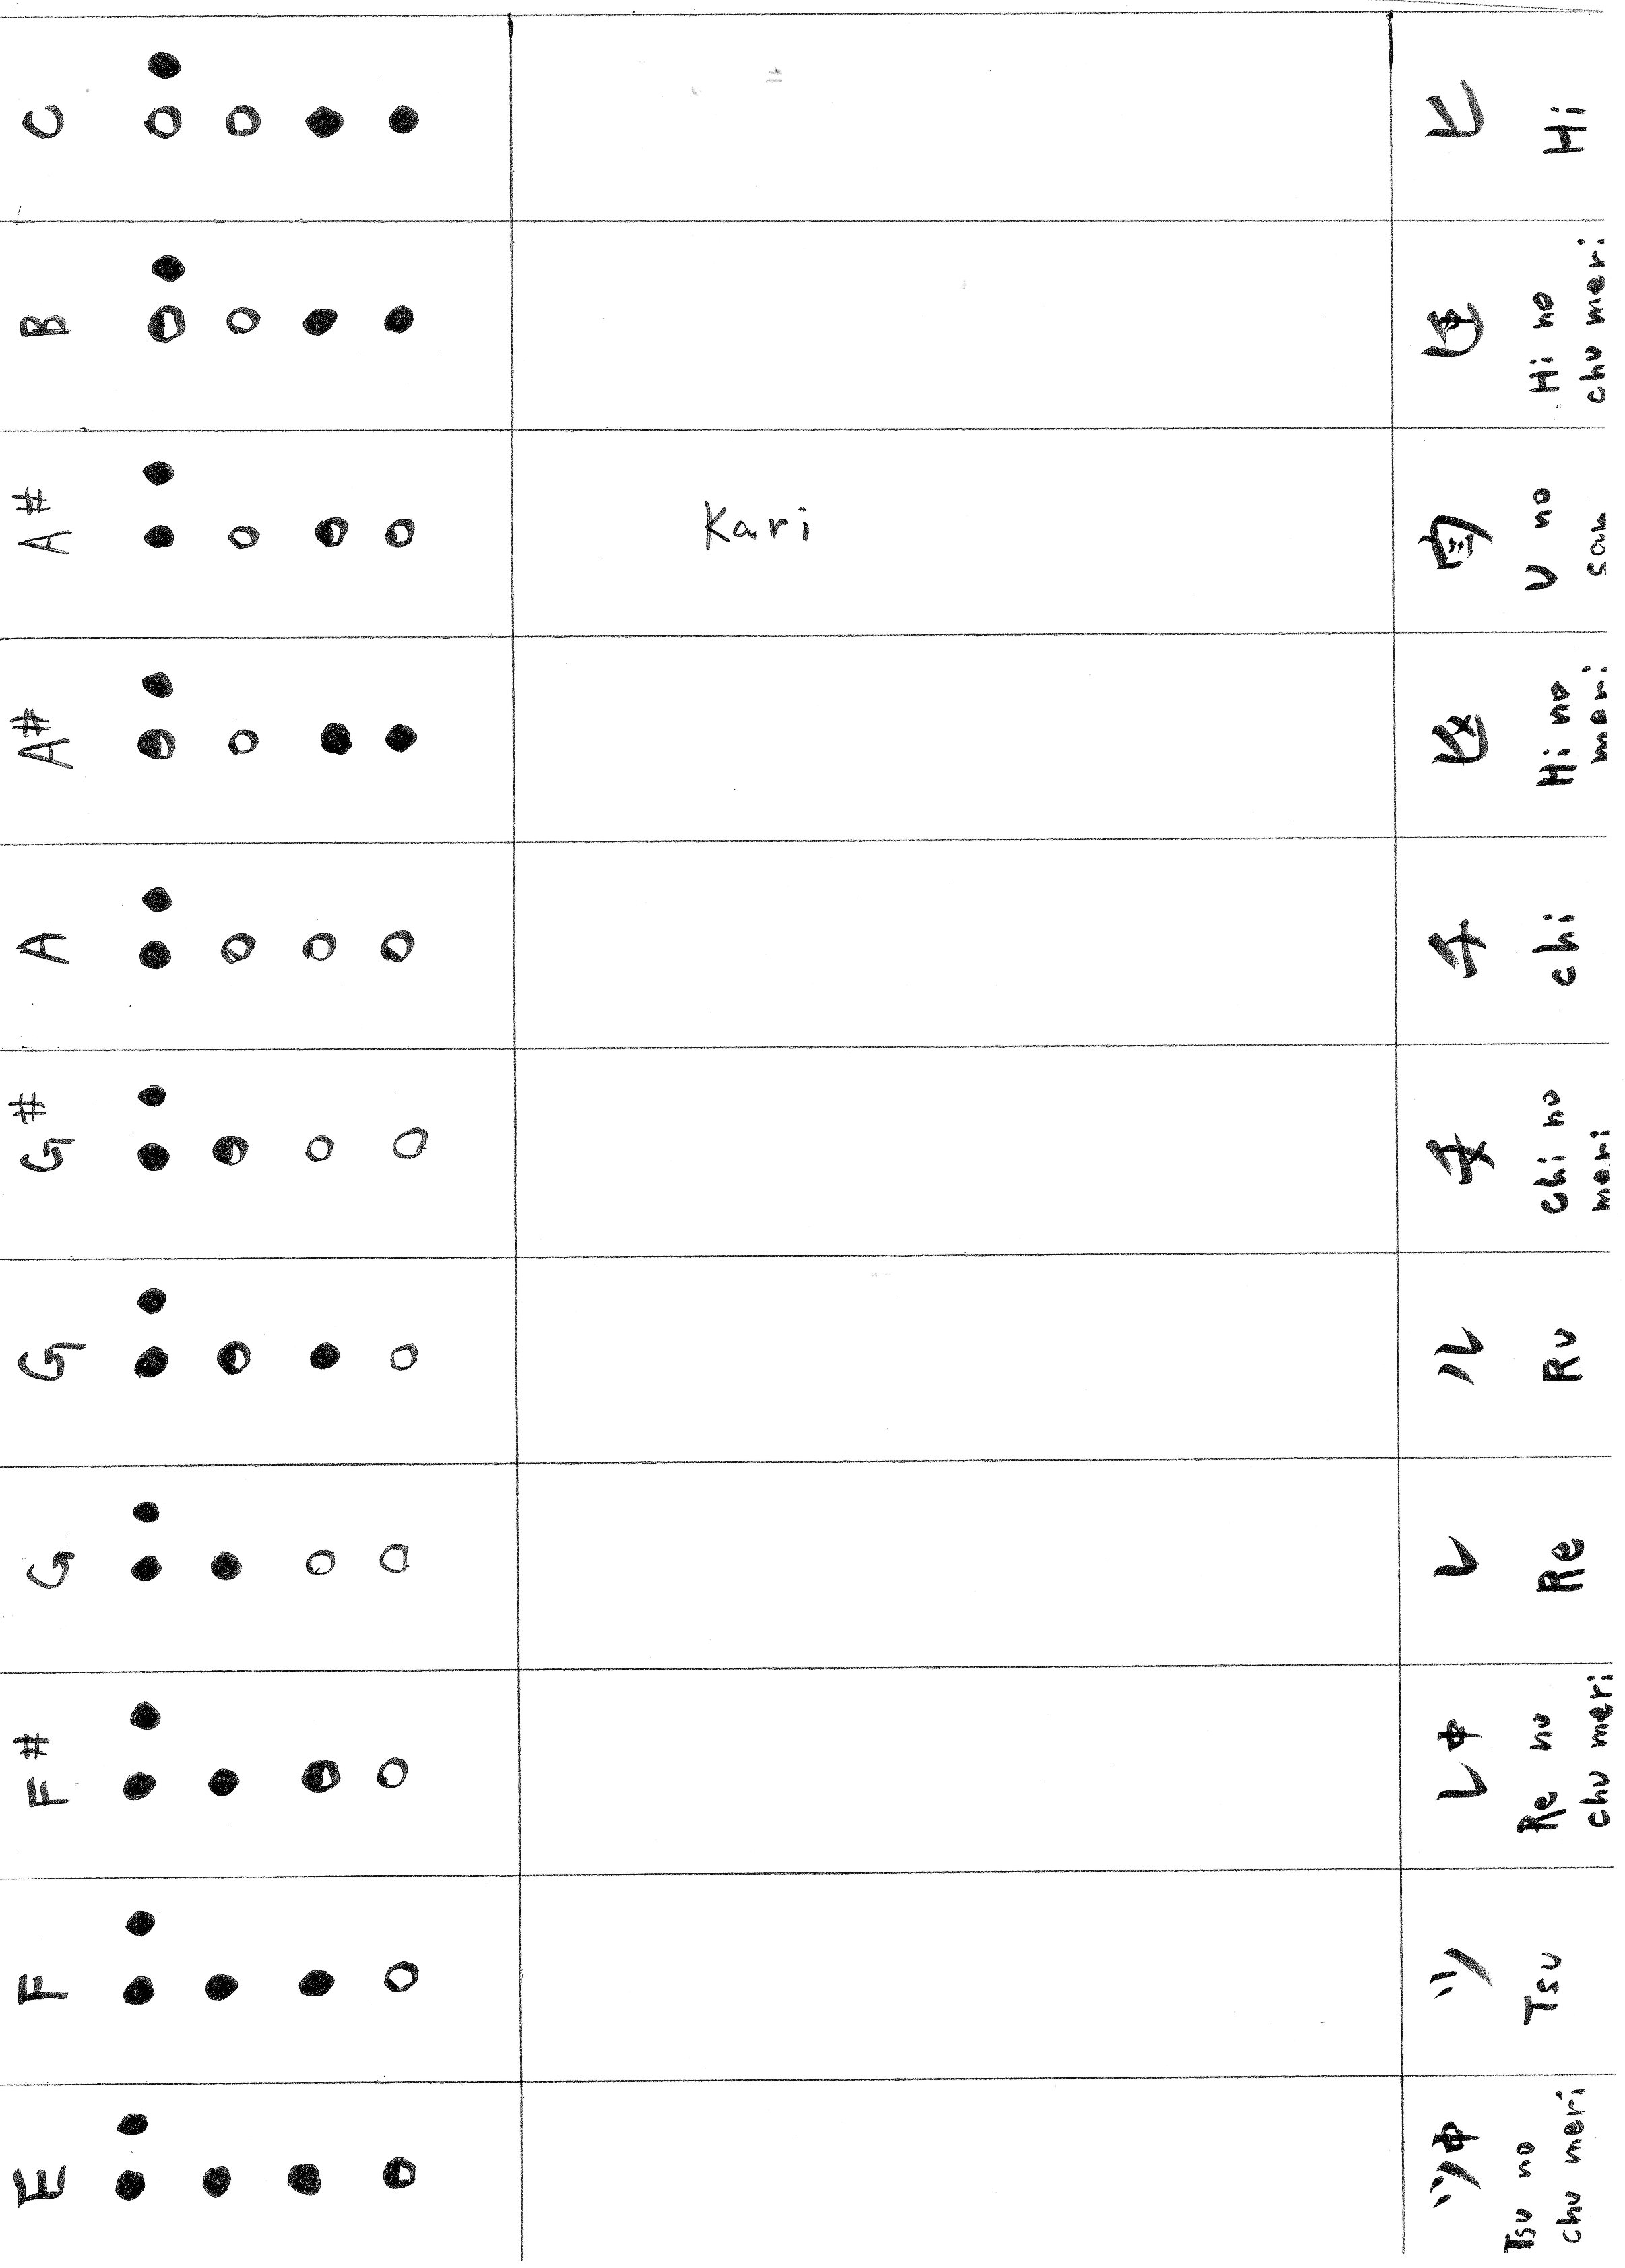
\includegraphics[width=0.8\textwidth,angle=270]{尺八の運指表3.jpg}
	% 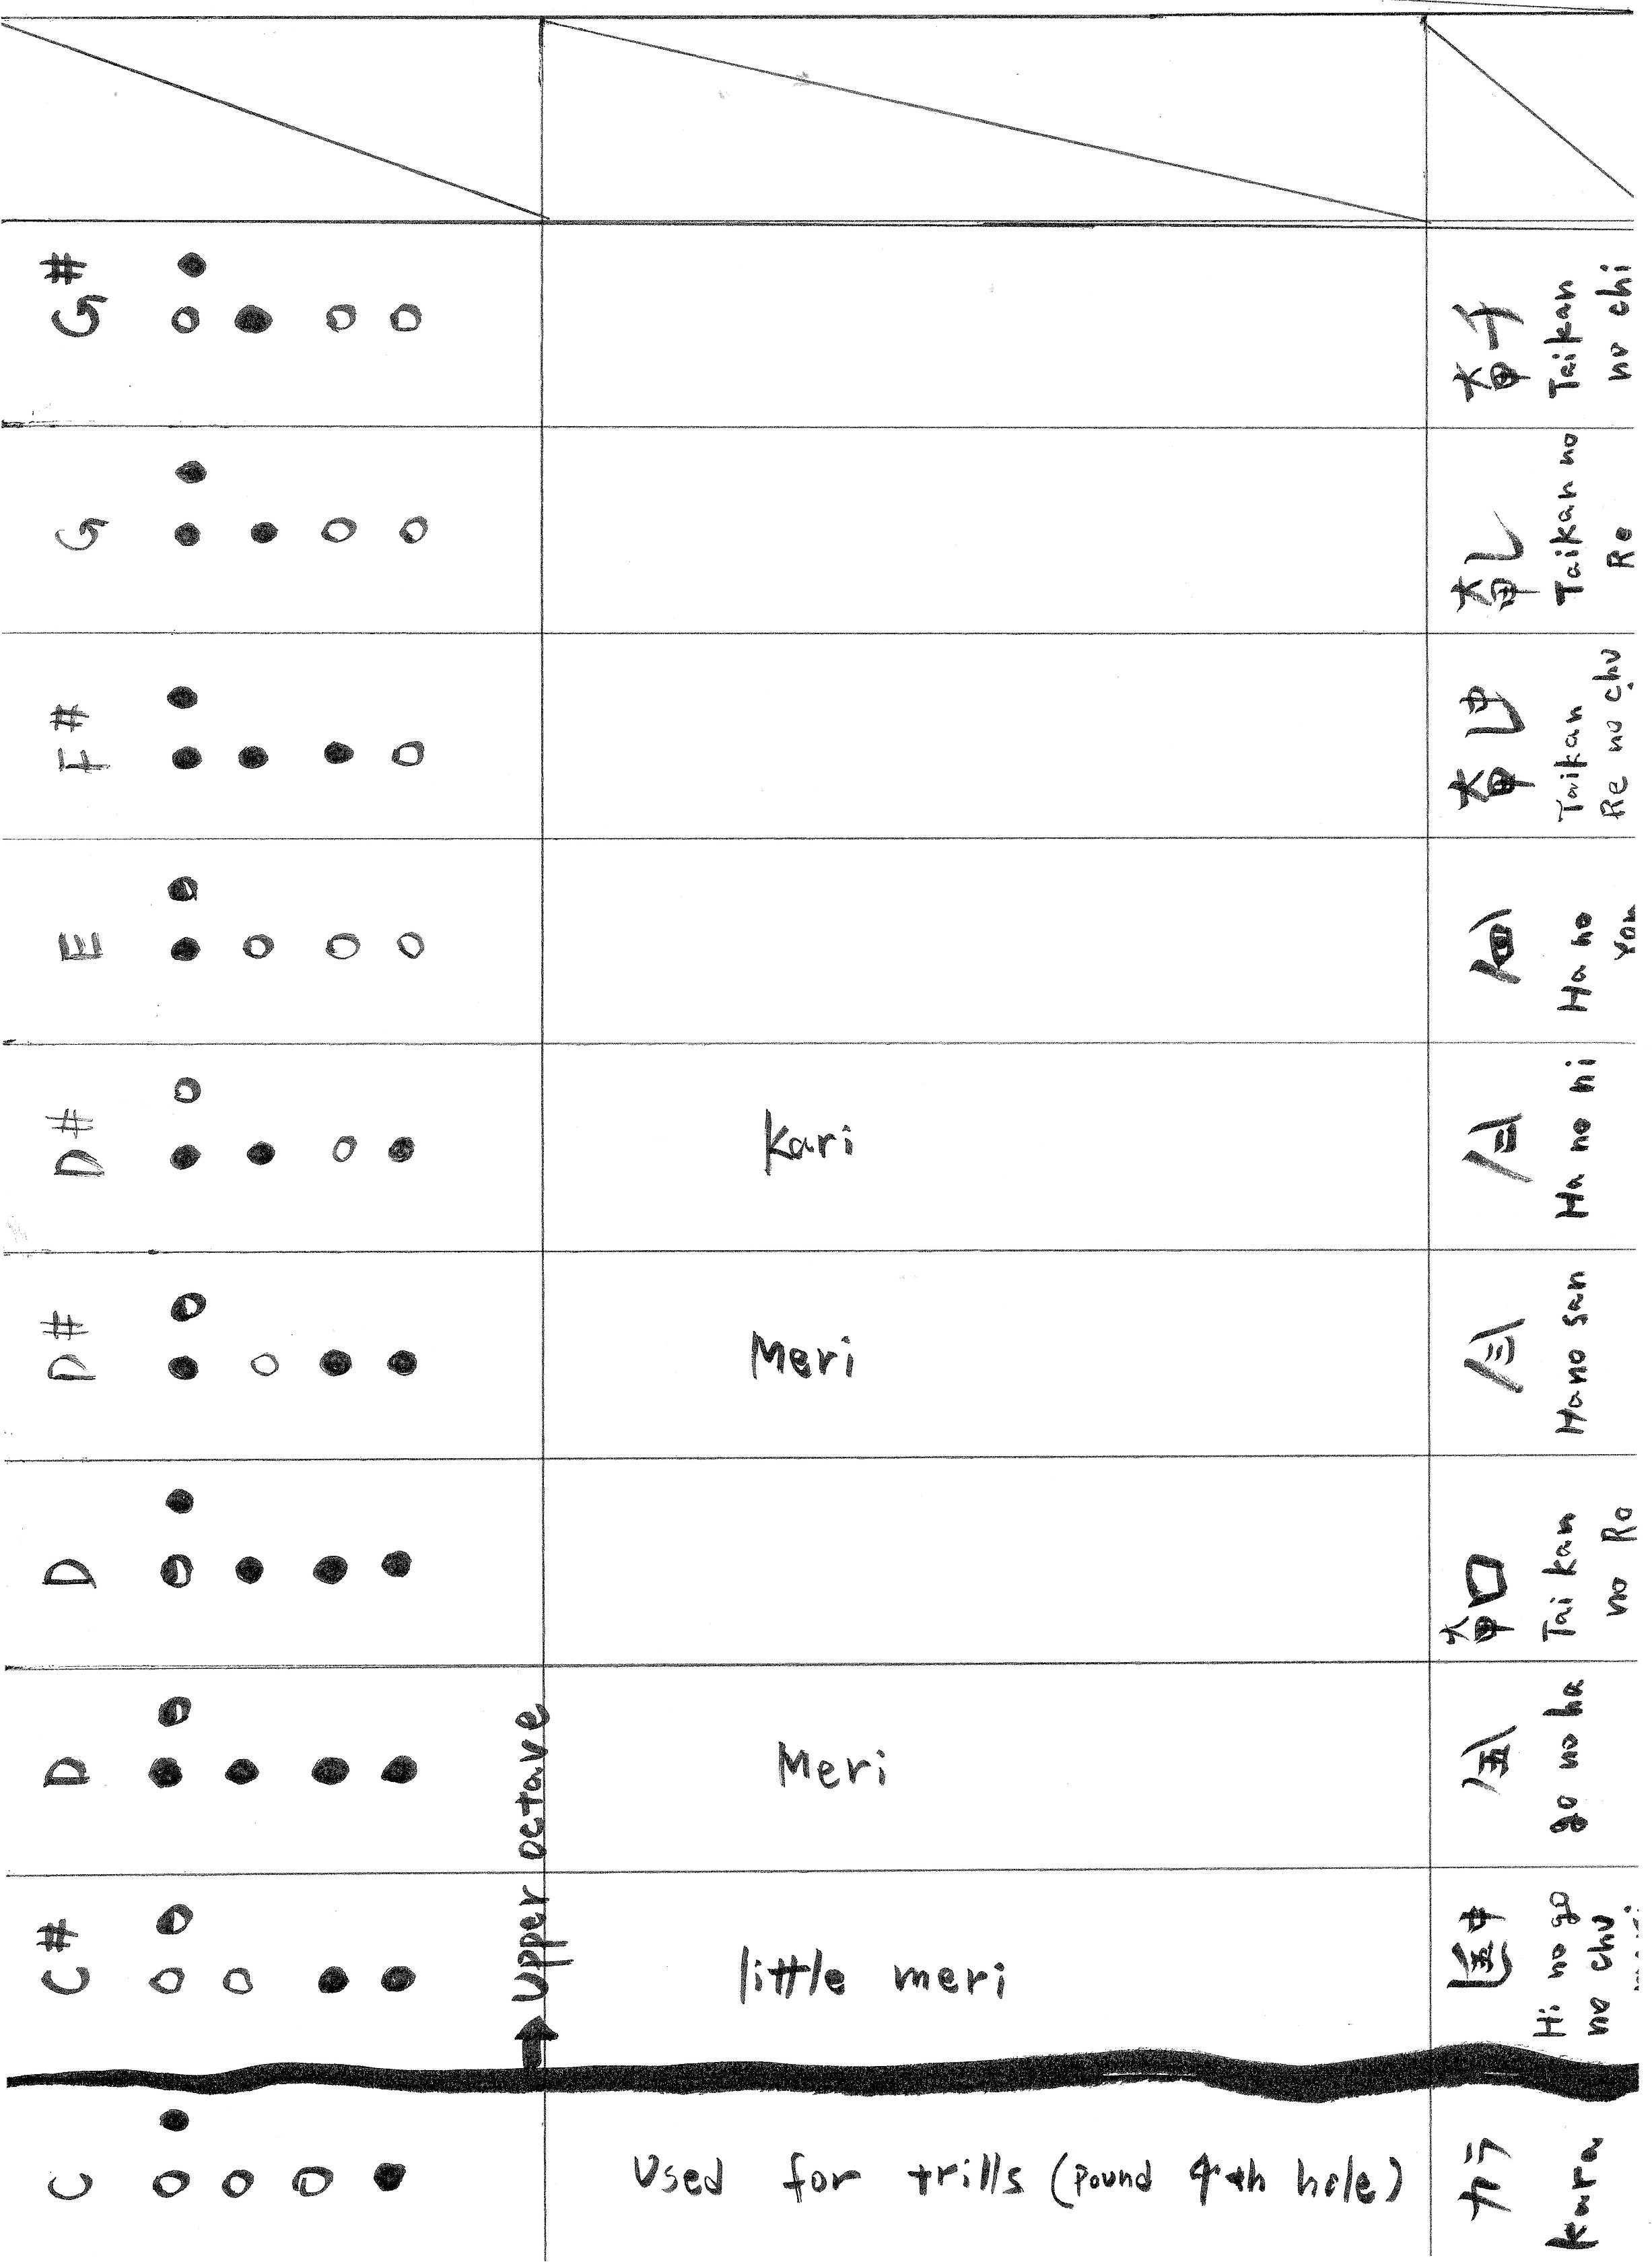
\includegraphics[width=0.8\textwidth,angle=270]{尺八の運指表4.jpg}
	\caption{Shakuhachi fingerings Part 2}
	\label{fig:shakuhachi_fingerings_2}
\end{figure}

\begin{figure}[p]
	\centering
	% 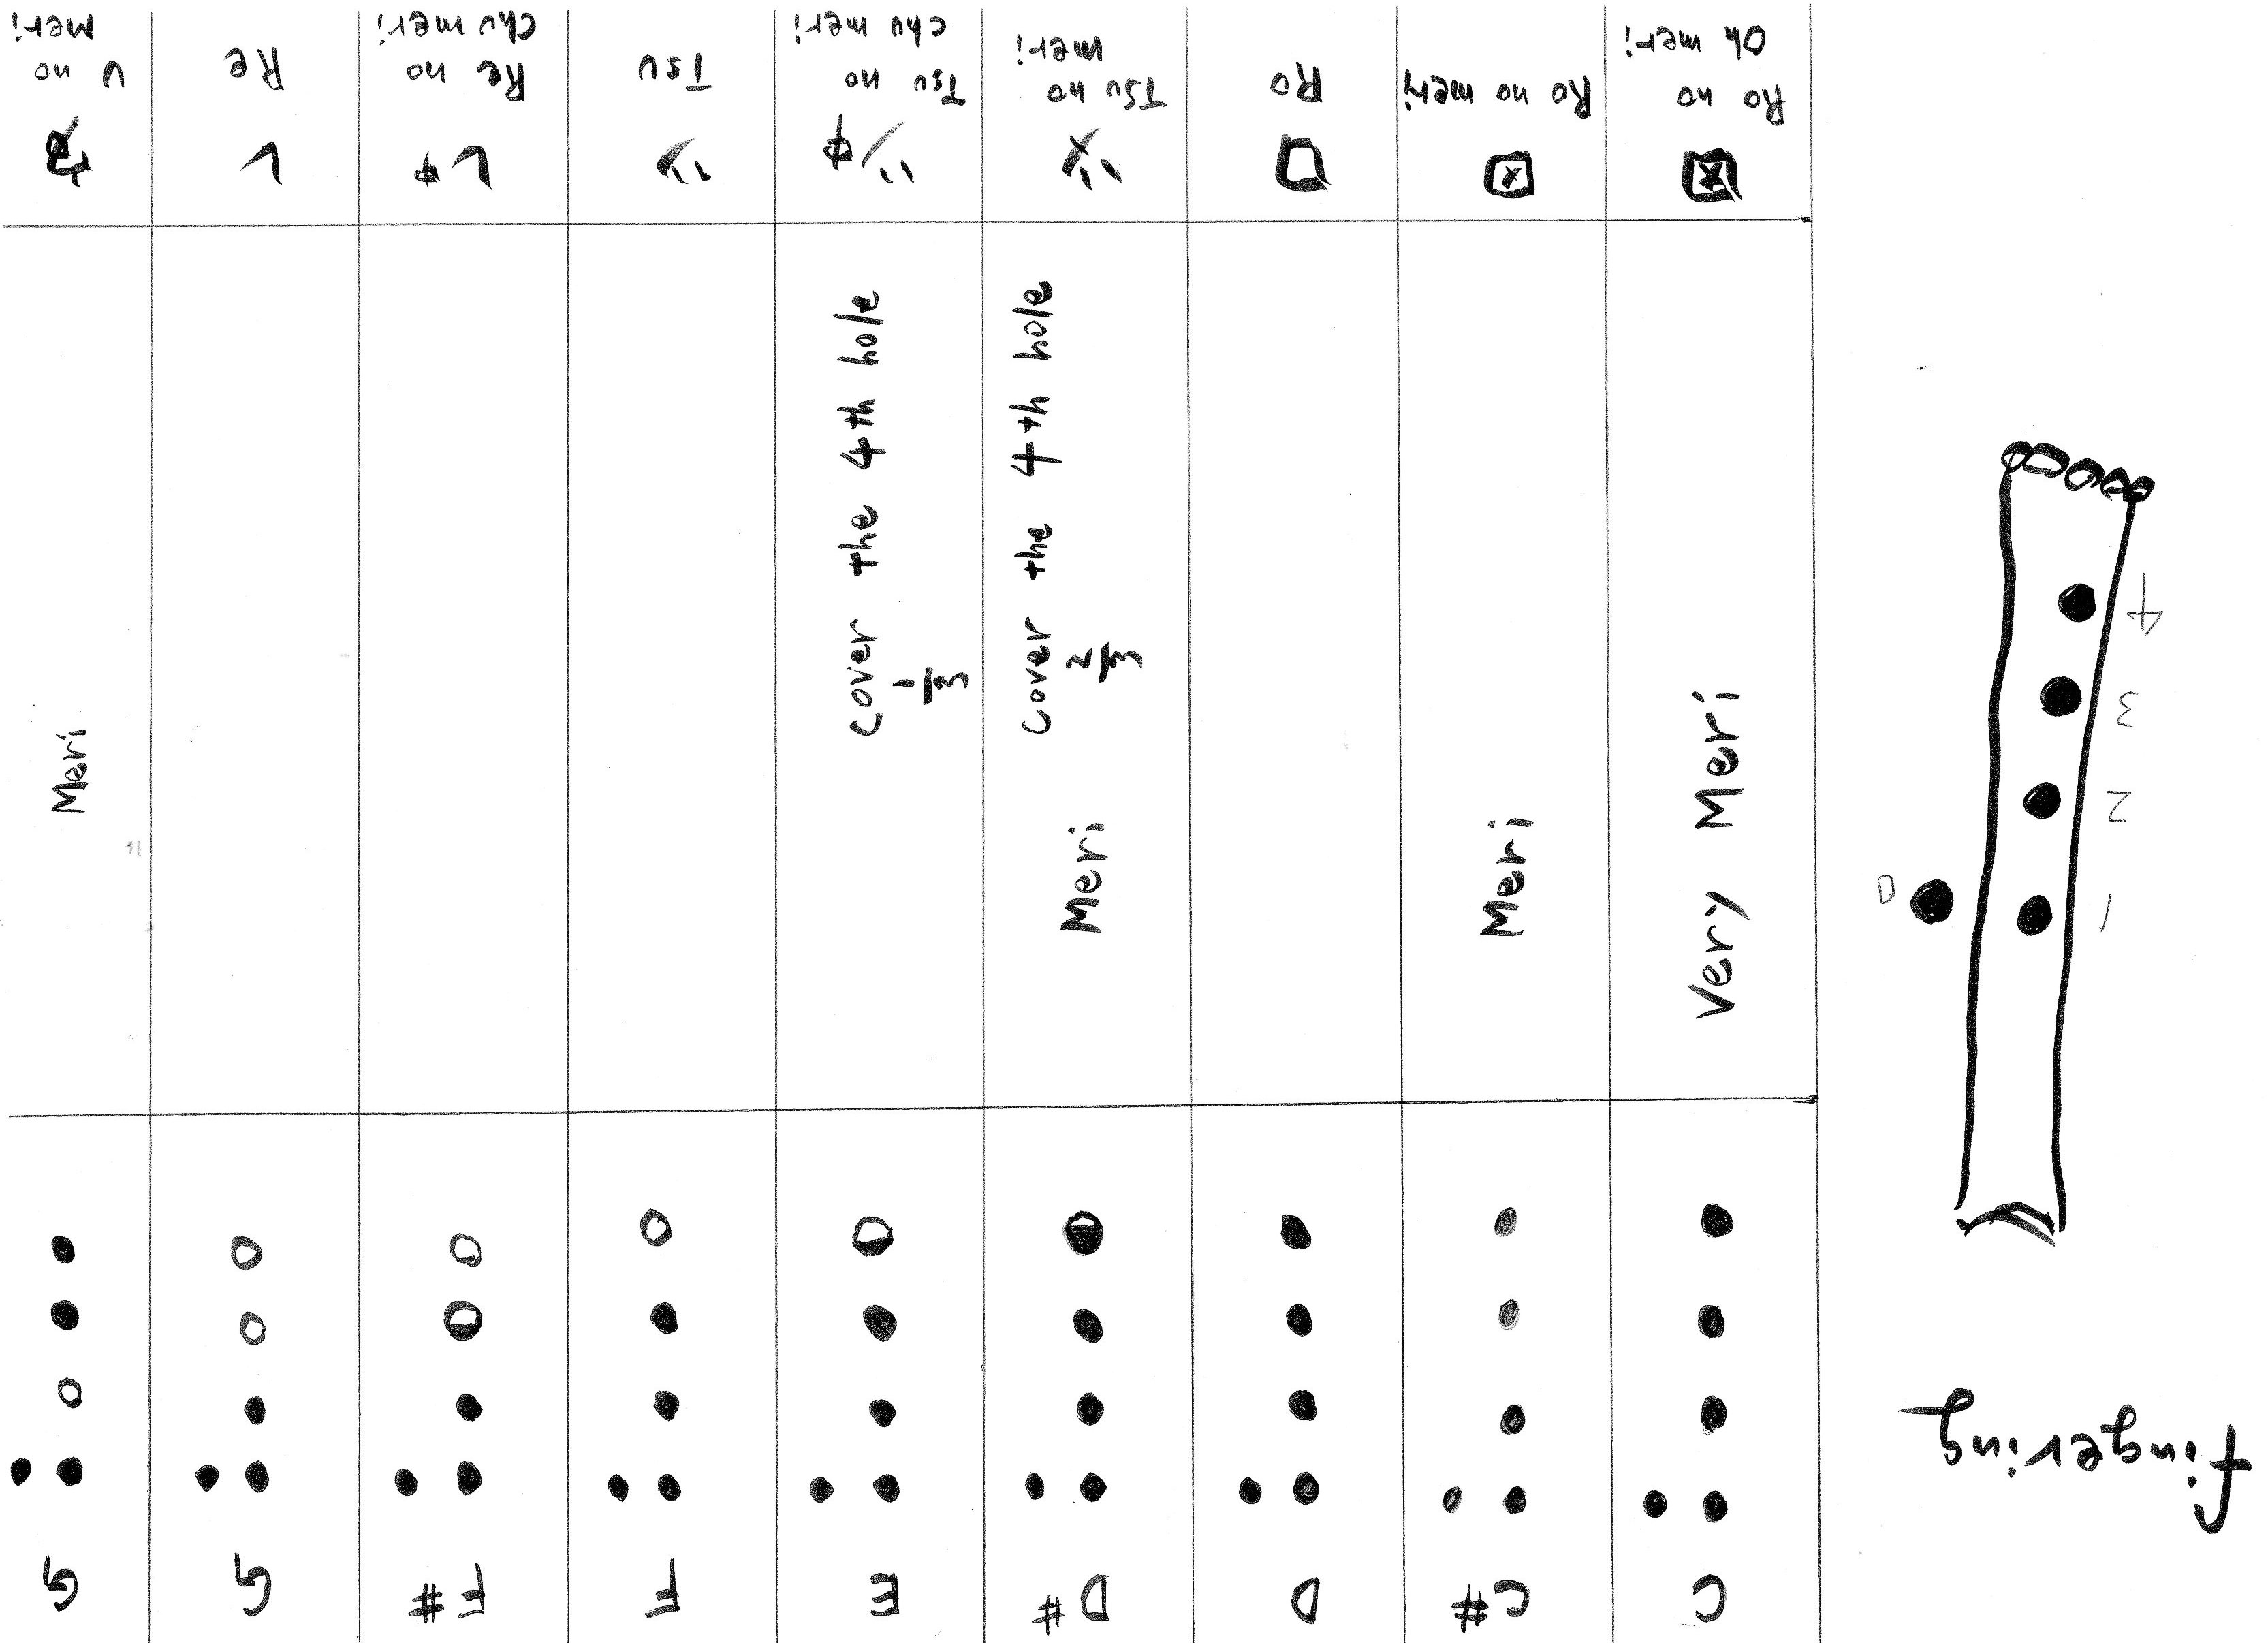
\includegraphics[width=0.8\textwidth,angle=270]{尺八の運指表1.jpg}
	% 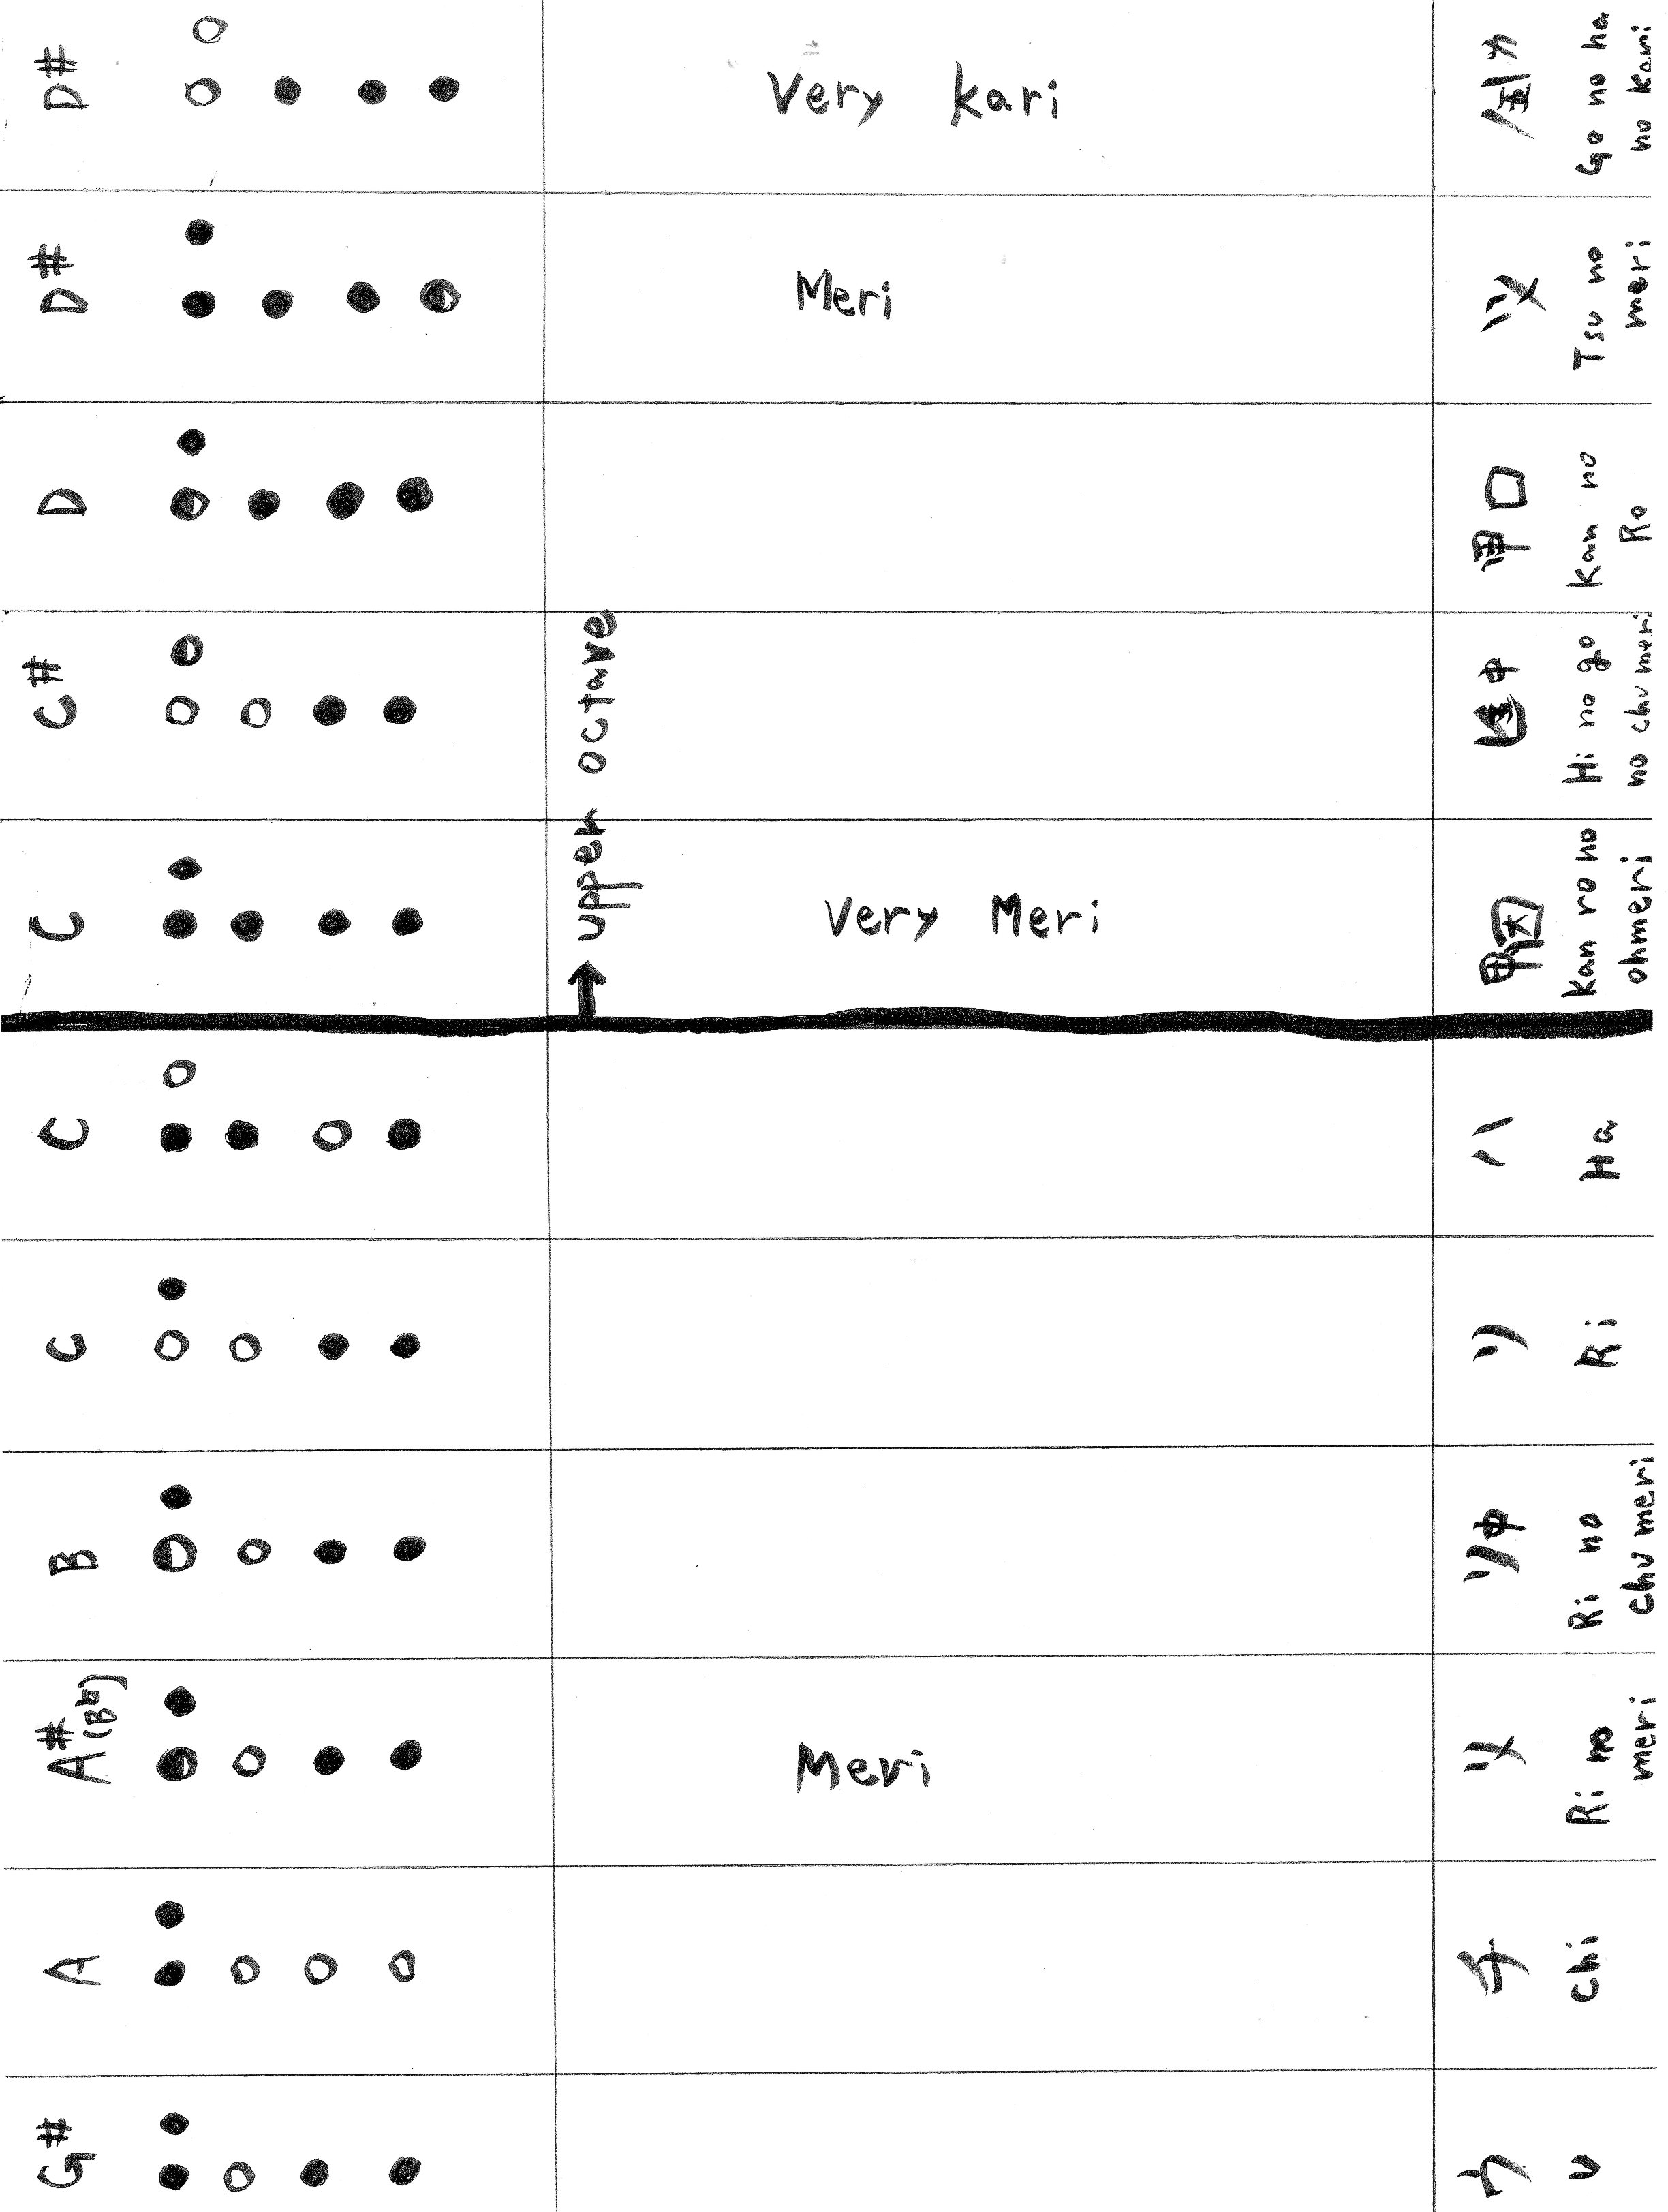
\includegraphics[width=0.8\textwidth,angle=270]{尺八の運指表2.jpg}
	% 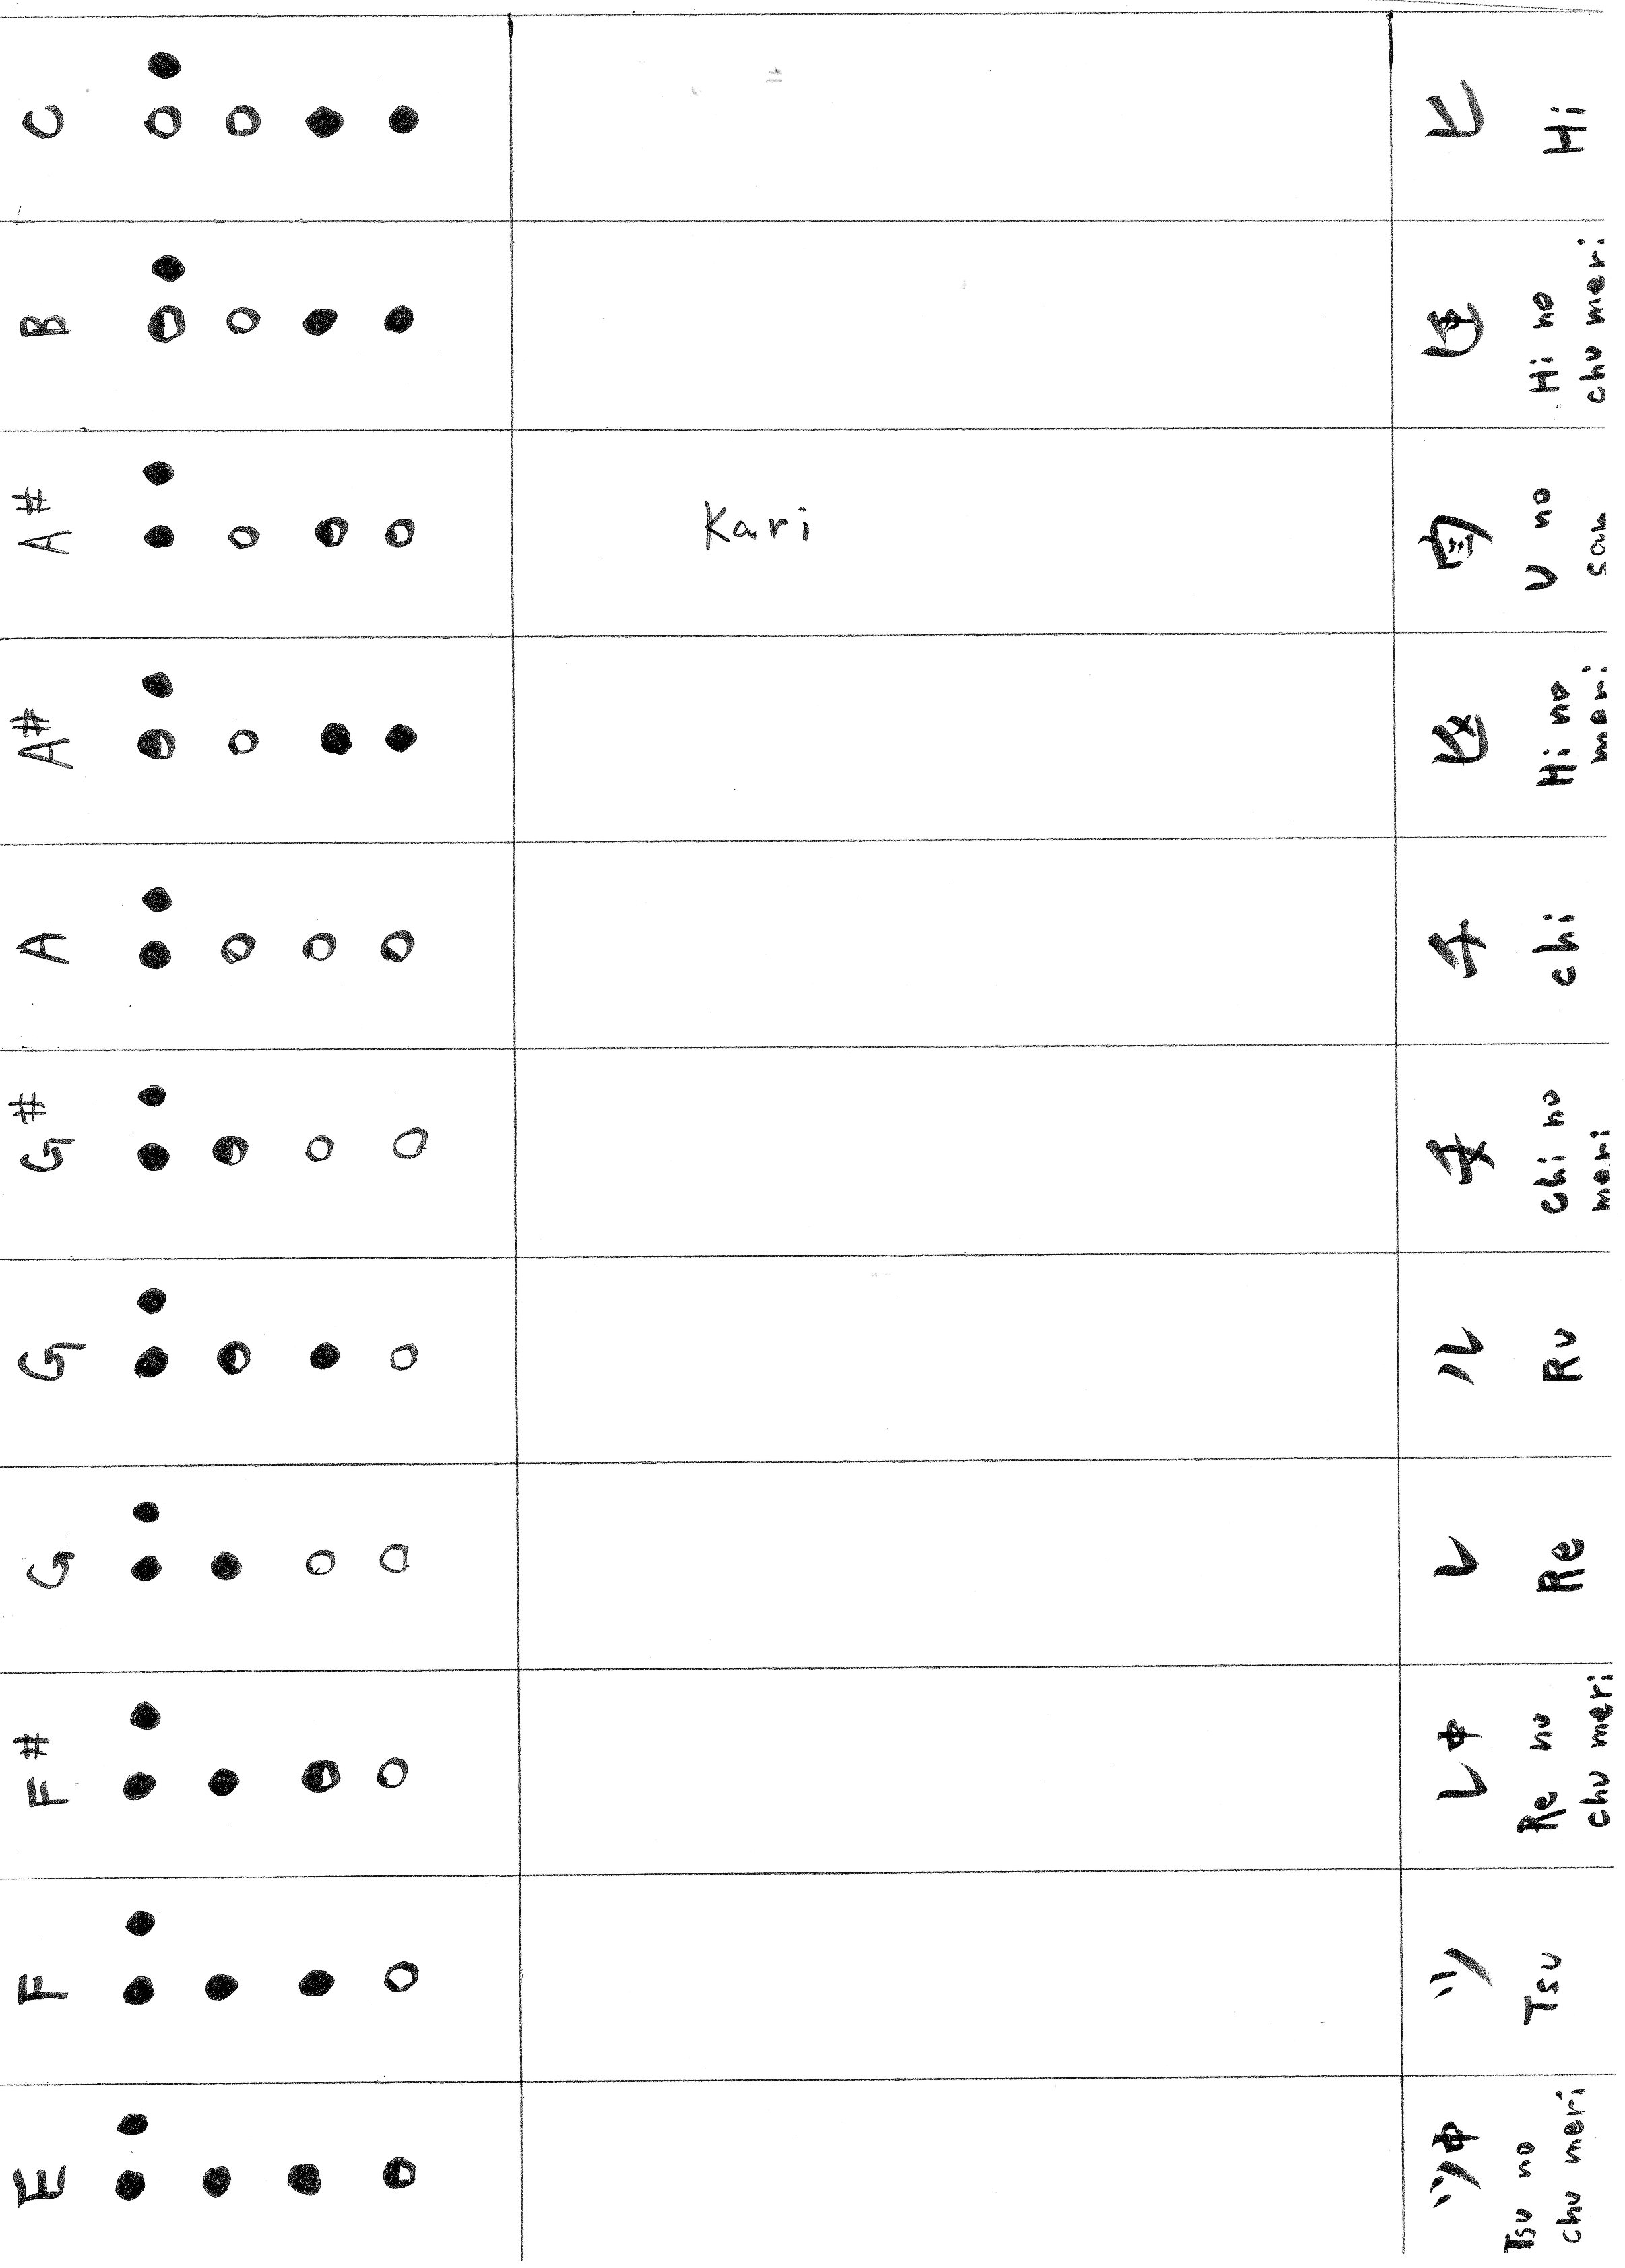
\includegraphics[width=0.8\textwidth,angle=270]{尺八の運指表3.jpg}
	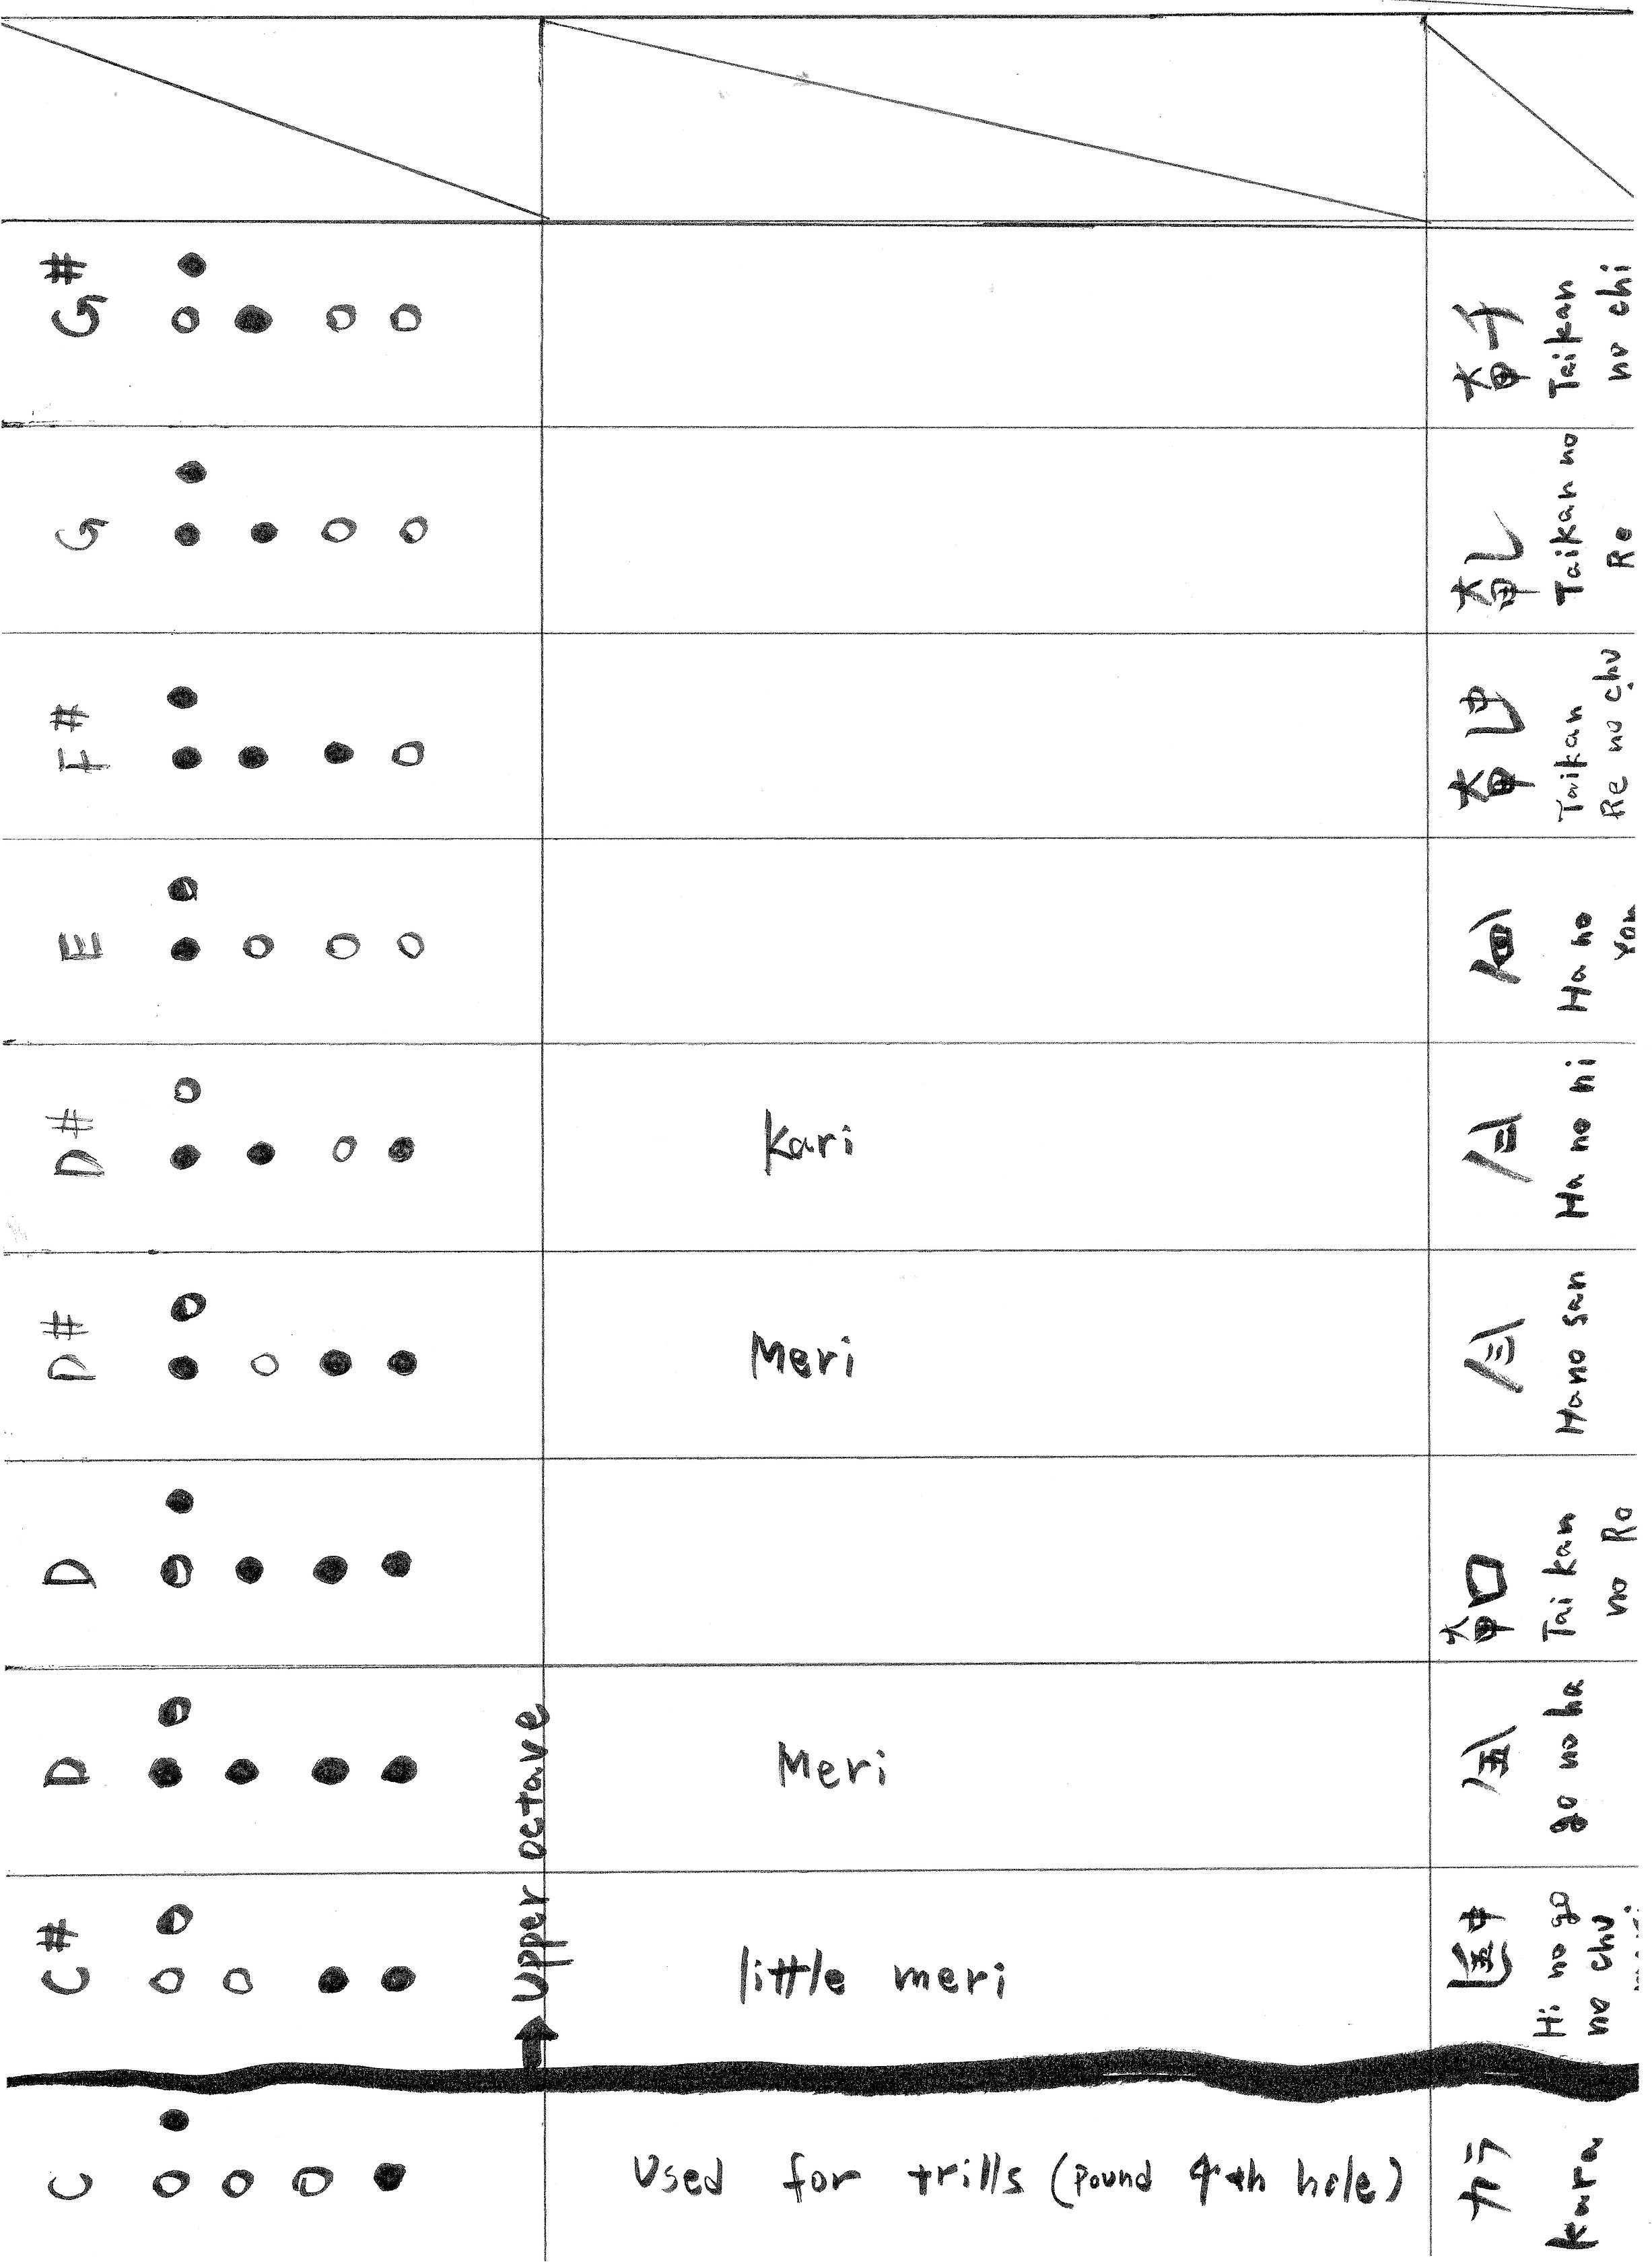
\includegraphics[width=0.8\textwidth,angle=270]{尺八の運指表4.jpg}
	\caption{Shakuhachi fingerings Part 3}
	\label{fig:shakuhachi_fingerings_3}
\end{figure}
